% % !TeX root = ../thuthesis-example.tex

\chapter{向量}

\section{线性表}

\textbf{线性表}是指相同类型的有限个数据组成的\textit{序列}。
本书按照邓书的方法,将线性表分为\textbf{向量}(vector)和\textbf{列表}(list)两种形式~\cite{邓俊辉2013数据结构},分别对应C++中的\lstinline{std::vector}和\lstinline{std::list}。
在另一些教材中,这两个词被称为\textbf{顺序表}和\textbf{链表}~\cite{严蔚敏1997数据结构},分别对应Java里的\lstinline{ArrayList}和\lstinline{LinkedList}。向量(顺序表)和列表(链表)这两对概念通常可以混用。
向量和列表代表着两种最基本的数据结构组织形式:\textbf{顺序结构}和\textbf{链式结构}。在这一节,将首先让读者对这两种组织形式有一个基本的印象。

首先,我们思考这样的问题:抛开顺序结构或链式结构不谈,\textit{线性表}这个概念本身具有怎样的性质?这将会指导我们设计\lstinline{AbstractLinearList}这个类。

对比它的基类\lstinline{DataStructure}。一般的数据结构的定义中,“某种结构化的形式”,在线性表这里被具体化为了“序列”。既然是序列,那么它会具有头和尾,会具有“第$i$个”这样的概念;每个元素有它在序列上的“上一个”和“下一个”元素。这是一个朴素的想法,从数学角度容易理解。但从计算机的角度,请您思考这样的问题:“元素”应该用什么表示?我们应该如何找到序列中的一个元素呢?

把计算机中的内存想像为一座巨大的旅馆,线性表是一个居住在其中的旅游团。现在旅游团预定了一大片连续的房间,比如,从1000到1099,并且让第1个游客住在1000,第2个游客住在1001,以此类推,那么我们就很方便地可以知道第$i$个游客的房间号。这种情况下,我们只需要知道游客的序号,就能知道它们居住的房间号。

但并不是每个人都会按部就班地居住,一些人可能喜欢阳光,一些人可能想和伙伴们做邻居,于是,这些游客开始交换房间。房间被交换之后,我们再也无法直接知道第$i$个游客的房间号。一个可能的想法是,从1000到1099每一个房间都敲敲门。这种方法虽然可行,但无疑是很低效的。

更加糟糕的是,旅游团可能没订到连续的房间,游客们散落在旅馆的各处。因为我们不可能像推销员那样每个房间都敲门(这会被赶出去的),所以再也无法找到我们想要的第$i$个游客了。为了应对这种情况,旅游团的导游往往会记录下各个游客所在的房间号,以便能够找到他们。

在上面这个比喻中,我们可以看到,如果数据结构中的元素被连续地储存,那么我们可以通过它们的序号(在邓书中,称为秩,rank)来找到它们;如果数据结构中的元素并没有被连续地储存,则我们只能通过它们的位置(position)来找到它们。上面的三种情况,分别是地址连续、且地址和秩相关的顺序结构(向量);地址连续、但地址和秩无关的静态链式结构(静态链表);地址不连续、也和秩无关的动态链式结构(动态链表)。图\ref{fig:vec1}示意了三种结构的区别。

\begin{figure}
  \centering
  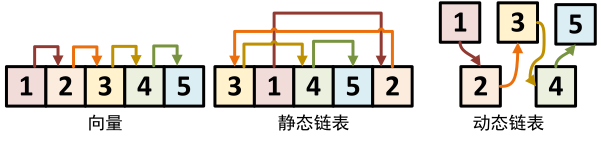
\includegraphics[width=0.8\linewidth]{figures/vec1.pdf}
  \caption{向量、静态链表和动态链表的对比}
  \label{fig:vec1}
\end{figure}

显然,如果发生了第二种情况,导游通常还是会选择记录房间号而不是逐个敲门。那么既然没有省事,也就没有必要预定一大片房间了。因为旅馆老板,也就是操作系统,可能会乘机宰客。比如,旅游团一次定了100个房间,但中途有50人提前结束了旅行。由于旅游团定的是整单,老板不允许单独退这50个人的房间。于是,旅游团要么承担50间空房的代价(空间损失);要么再定50个房间,请剩下的50人搬到新房间住(时间损失),然后把原来的100个房间一并退掉。

这个例子展示了静态链表是一个不实用的数据结构,因此在邓书中它被删除。在包括静态链表的教材中,它也不是重点的一部分。我们将聚焦在向量和动态链表(列表)上。
如前所述,向量和列表里定位元素的方法是不同的。向量是循秩访问,而列表则循位置访问。因此,我们设计的线性表抽象类中需要反映这一点。

\begin{lstlisting}
template <typename T, typename Pos>
class AbstractLinearList : public DataStructure<T> {
public:
    virtual T& get(Pos p) = 0;
    virtual void set(Pos p, const T& e) = 0;

    virtual Pos insert(Pos p, const T& e) = 0;
    virtual Pos find(const T& e) const = 0;
    virtual T remove(Pos p) = 0;
    virtual void clear() = 0;
};
\end{lstlisting}

如果您查看AbstractLinearList.ixx,还会看到一些其他的方法。正如序言中所说的那样,那些和《数据结构》研究的内容关系不大的方法将在书里被隐藏。上面的代码中只展示了一些重要的方法。

\begin{enumerate}
    \item 根据位置$p$,访问或修改在位置$p$上的元素。
    \item 将元素插入到位置$p$上。
    \item 在线性表中查找一个给定的元素,返回它所在的位置。
    \item 删除位置$p$上的元素,以及将整个线性表清空。
\end{enumerate}

\textit{您可能会觉得,这个线性表类中包含的内容过多或者过少。如果您感兴趣,我也非常鼓励您实现自己的抽象类模板。本书给出的模板保证您在不参与设计细节的情况下能完成本书设计的有趣实验,您可以随时用自己实现的程序替换其中的一部分。如果您打算这么做,请记得使用版本控制程序或备份,保证您可以回退到程序能正常运行的时刻。}

\section{向量的结构}

\textbf{向量}(vector)是一个基于\textbf{数组}(array)的数据结构,它在内存中占据的是一段连续的空间。C++建议更多地使用标准库中的向量\lstinline{std::vector}代替数组。向量和数组相比,其最重要的区别在于它是运行时\textit{可变长的},而在其他使用上,二者基本可以等同。因此,向量上的算法可以很容易地修改为数组上的算法(即使不使用\lstinline{std::span})。在408中通常不考虑可变长这一性质,此时讨论的顺序表就是数组,但您同样可以用本章中介绍的向量算法解决相关题目。

作为一种基于数组的线性表,\textit{向量的元素次序和数组的元素次序相同}。如果一个向量$V$基于长度为$n$的数组$A$构建,那么向量$V$的第$i$个元素就是$A[i]$。我们知道,C语言的数组可以视为指针,于是向量$V$的第$i$个元素的地址就是$A+i$。

向量里的元素数量$n$,称为向量的\textbf{规模}(size);而向量所占有的连续空间能够容纳的元素数量$m$,称为向量的\textbf{容量}(capacity)。这两者通常是不同的,规模必定不大于容量,而在不超过容量的前提下,向量的规模可以灵活变化,从而赋予了它比数组更高的灵活性。
前面的那个旅行团的例子也可以帮助理解规模和容量的关系。一个$n$个人的旅行团订了连续的$m$个房间,这里$m$可以大于$n$,这样,如果旅行过程中有新人加入团队,他们就可以直接加入到已经预定的连续房间中来。

\begin{figure}
  \centering
  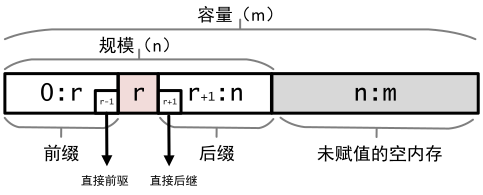
\includegraphics[width=0.8\linewidth]{figures/vec2.pdf}
  \caption{向量的基本概念}
  \label{fig:vec2}
\end{figure}

如图\ref{fig:vec2}所示,
对于向量中的每一个元素$V[i]$来说,它前面的元素称为它的\textbf{前驱}(predecessor),它后面的元素称为它的\textbf{后继}(successor)。特别地,和它位置相邻的前驱,也就是\textbf{直接前驱}为$V[i-1]$,相应地,\textbf{直接后继}为$V[i+1]$。所有的前驱构成了\textbf{前缀}(prefix),也就是$V[0$:$i]$;所有的后继构成了\textbf{后缀}(suffix),也就是$V[i+1$:$n]$。本书中我们用$V[a$:$b]$来简记$V[a],V[a+1],\dots,V[b-1]$这个子序列,这是Python的切片(slice)语法,借助它可以简化很多叙述,尤其在记忆一些比较复杂的算法时很有用。

\section{循秩访问}

了解了向量的定义之后,我们将之前实现的线性表抽象类进行细化,构建向量的抽象类\lstinline{AbstractVector}。随后本书会讲解一个示例实现,您可以自行继承\lstinline{AbstractVector}进行实现,因为那些不需要您关注的方法都已经在这个抽象类中实现。\textit{比如说迭代器,对于读者而言实现迭代器会花费比较多的时间,因此,尽管示例代码中实现了一个迭代器以使我们的向量能够支持STL里的算法,但迭代器被排除在基本实验体系之外。我们的目标是学习数据结构,而不是复现STL。}如果您感兴趣,可以自己查看示例代码进行学习;也欢迎您为本书的示例代码提出建议。

向量的核心特征是\textbf{循秩访问}。称元素$V[i]$在向量$V$中的序号$i$为它的\textbf{秩}(rank)。对于建立在数组$A$上的向量$V$,因为$V$和$A$的元素次序是一致的,所以$V[i] = A[i] = *(A+i)$。因此,只要知道一个元素的秩,就可以在$O(1)$的时间内访问该元素。
通常,我们用\lstinline{size_t}类型存储下标。为了强调向量是循秩访问的,我们给它一个别名。

\begin{lstlisting}
using Rank = size_t;
\end{lstlisting}

接下来,我们开始构筑向量抽象类。首先,除了在\lstinline{DataStructure}里定义的规模\lstinline{size}之外,我们还需要定义容量\lstinline{capacity}。同时,因为向量是可变长的,所以规模和容量都是可以变化的,还需要两个修改它们的方法。有了修改规模的方法,线性表里的\lstinline{clear}就可以直接用\lstinline{resize(0)}实现。其次,我们需要构筑循秩访问的体系,重写\lstinline{AbstractLinearList}里面的\lstinline{get}和\lstinline{set}方法。

\begin{lstlisting}
template <typename T>
class AbstractVector : public AbstractLinearList<T, Rank> {
protected:
    virtual T* data() = 0;
public:
    virtual size_t capacity() const = 0;
    virtual void reserve(size_t n) = 0;
    virtual void resize(size_t n) = 0;
    
    T& get(Rank r) override {
        return data()[r];
    }
    void set(Rank r, const T& e) override {
        data()[r] = e;
    }
    void clear() override {
        resize(0);
    }
};
\end{lstlisting}

操作底层内存的时候,因为和所有权无关,所以不能使用智能指针,只能使用裸指针。为了避免裸指针被外部获取,我们将向量的获取首地址方法\lstinline{data()}设置为受保护的,而公共方法只会返回引用。

现在,我们已经拥有了一个抽象类\lstinline{AbstractVector},它还缺少下面这些组件的实现:获取规模、容量和首地址的方法;修改规模和容量的方法;插入、删除、查找的方法。如果您打算自己实现向量类,只需要在抽象类的基础上补充它们即可;您也可以继承本书提供的示例向量类,重写其中的部分方法。我们的示例类会从下面开始。

\begin{lstlisting}
template <typename T>
class Vector : public AbstractVector<T> {
    std::unique_ptr<T[]> m_data { nullptr };
    size_t m_capacity { 0 };
    size_t m_size { 0 };

    T* data() override { return m_data.get(); }
public:
    size_t capacity() const override { return m_capacity; }
    size_t size() const override { return m_size; }
}
\end{lstlisting}

C++14起,允许用户使用智能指针管理数组,因此我们使用\lstinline{std::unique_ptr}来申请内存。它的主要好处是不需要在析构函数里手动释放,减少了手动管理内存的麻烦。本书中若无特殊情况,将总是使用智能指针来表示所有权,避免在任何地方使用\lstinline{delete}关键字释放内存。

\section{向量的容量和规模}
\subsection{初始化}

当我们建立一个新的数据结构的时候,有几种情况是比较典型的。在这里,以向量为例展示它们,后面讨论其他的数据结构的时候不再赘述。

\textbf{零初始化}。即,生成一个空的数据结构。对于向量来说,这应该包含一个大小为0的数组,并把容量和规模都赋值为0。然而,C++不支持大小为0的数组,所以只能把\lstinline{data}赋值为\lstinline{nullptr},就像在上一节中展示的默认值那样。

\textbf{指定大小的初始化}。即,给定$n$,生成一个规模为$n$的数据结构,其中的每个元素都采用默认值(即元素采用零初始化)。对于向量而言,可以申请一片大小为$n$的内存,如下面的代码所示。

\begin{lstlisting}
Vector(size_t n) : m_data { std::make_unique<T[]>(n) }, m_capacity { n }, m_size { n } {}
\end{lstlisting}

\textbf{复制初始化}。即,给定相同数据结构的一个对象,复制该对象里的所有数据及数据之间的结构化关系。对于向量来说,只需要在申请大小为$n$的内存之后,将给定的向量的元素逐一复制进来即可,如下面的代码所示。注意这里在初始化器中显式调用了上面的“指定大小的初始化”的构造函数,为向量进行了初步的初始化,然后再把另一个向量的数据复制进来。

\begin{lstlisting}
Vector(const Vector& rhs) : Vector(rhs.m_size) { std::copy_n(rhs.m_data.get(), rhs.m_size, m_data.get()); }
\end{lstlisting}

\textbf{移动初始化}。即,给定相同数据结构的一个对象,将该对象里的所有数据及数据之间的结构化关系移动到当前对象处。\textbf{移动}(move)语义和复制(copy)有显著的不同,因为在移动之后,“被移动”的对象失去了对数据的所有权,我们永远不会从被移动后的对象里访问那些数据。下面展示了向量移动初始化的一个例子。

\begin{lstlisting}
Vector(Vector&& rhs) noexcept : m_data { std::move(rhs.m_data) }, m_capacity { rhs.m_capacity }, m_size { rhs.m_size } {
    rhs.m_capacity = 0;
    rhs.m_size = 0;
}
\end{lstlisting}

通过对智能指针调用\lstinline{std::move},我们可以在常数时间内,将被移动对象的数据转移到新对象里。可以看出,被移动之后,\lstinline{rhs}的数据区被复位为空指针,规模和容量都被置0,就像它被零初始化了一样,成为了一个空向量。

\begin{figure}
  \centering
  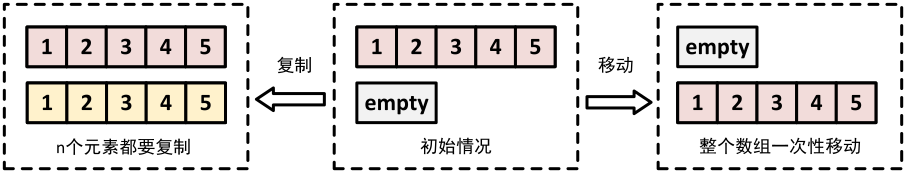
\includegraphics[width=\linewidth]{figures/vec3.pdf}
  \caption{复制和移动的区别}
  \label{fig:vec3}
\end{figure}

从图\ref{fig:vec3}中可以直观了解到复制和移动的语义区别。当数据结构里的元素数量很多时,逐元素地复制是一项复杂、琐碎、漫长的工程,而移动则是一项简单、整体、快速的工作。在本书的示例代码中,我们经常会给同一个函数提供一个复制版本和一个移动版本。比如,对于插入(insert),我们定义一个插入\lstinline{const T&}类型的方法用于复制(不破坏源),又定义了一个插入\lstinline{T&&}类型的方法用于移动(破坏源)。这些方法之间往往只有一个或几个\lstinline{std::move}的区别,因此本书通常省略移动版本的方法,而只展示复制版本的方法。尽管如此,在您的日常编程中需要时刻注意,只要复制和移动的时间成本\textit{有可能}相差比较远,就应该同时定义并实现复制和移动两个版本的方法,而不能只实现复制。

需要注意的是,析构函数、复制构造函数、移动构造函数、复制赋值运算符、移动赋值运算符这5个函数,一旦显式定义其中的一个(比如想要定义复制构造函数),编译器就不会生成其他的函数。处于“一荣俱荣,一损俱损”的关系。因此,我们在日常编程的时候,通常选择不实现它们中间的任意一个函数(0原则,rule of zero),因为日常编程的时候,通常都使用的是STL对象,而STL里已经将这些功能实现了。但是,在我们实现一些比较底层的结构时候,没法依靠STL里的实现,需要实现这5个函数中的一个或几个。此时,就必须要将所有的5个函数实现(5原则,rule of five)。我们可以使用\lstinline{=default}来显式使用自动生成的函数,但如果我们不显式说明它,这些函数将不会被包含在这个类中。

\textbf{初始化列表初始化}。即,使用初始化列表\lstinline{std::initializer_list}对数据结构进行初始化。初始化列表也是一个典型的线性容器,可以直接使用STL方法复制。

\begin{lstlisting}
Vector(std::initializer_list<T> ilist) : Vector(ilist.size()) { 
    std::move(ilist.begin(), ilist.end(), m_data.get()); 
}
\end{lstlisting}

支持初始化列表初始化之后,我们就可以用下面的形式来初始化一个向量。
\begin{lstlisting}
Vector V {1, 2, 3};
\end{lstlisting}

\subsection{装填因子}
设向量的容量为$m$,规模为$n$,则称比值$\frac{n}m$为\textbf{装填因子}(load factor)。正常情况下,这是一个$[0,1]$之间的数。装填因子是衡量向量效率的重要指标。

\begin{enumerate}
    \item 如果装填因子\textit{过小},则会造成内存浪费:申请了巨大的数组,但其中只有少量的单元被向量中的元素用到,其他单元都被闲置了。
    \item 如果装填因子\textit{过大}(超过1),则会引发数组越界,造成\textit{段错误}(segmentation fault)。
\end{enumerate}

刚开始的时候,装填因子一定是在$[0,1]$之间的。
但因为数组的容量$m$是固定的,而向量的规模$n$是动态的,所以一开始分配的$m$可能后来会不够用,从而产生装填因子大于1的问题,此时就需要令$m$增大,这一操作称为\textbf{扩容}(expand)。\textit{由于408不讨论变长顺序表的问题,所以下面的几个章节可以略读。}

\subsection{改变容量和规模*}

您可能会想到,除了扩容之外,我们还可以进行\textbf{缩容}(shrink),降低$m$的值从而避免装填因子过小,造成内存浪费。但是,现实中很少进行缩容。因为扩容和缩容都需要时间,在扩容的场合是实现可变长特性的必需,但在缩容的场合仅仅是节约了空间而已。有多个原因让我们不愿意缩容:
\begin{enumerate}
    \item 我们可以接受一定程度的空间浪费,因为很少有程序能占满全部的内存。
    \item 如果缩容之后,又因为规模扩大而不得不扩容,一来一回浪费了不少时间,而价值甚微。
    \item 当不得不考虑空间时,我们有很多其他方法可以节约出这些空间,不一定要使用缩容的技术。比如复制初始化生成一个新向量,然后清空原向量来释放内存;按照之前介绍的方法,这个新向量的装填因子为1,处在空间最大利用的状态。
\end{enumerate}

因此,在本书中将不再讨论缩容;\textit{您可以在自己的向量类中实现这个特性,并观察它的效果}。

无论是扩容还是缩容,我们都需要重新申请一片内存。在扩容的场合,这很好理解。我们预定了1000到1099的房间,但在我们预定之后,1100号房间可能被其他旅客占用了。这时如果我们想要预定连续的200个房间,就需要重新找一段空房间。缩容的场合,则是为了安全性考虑,不允许释放数组的部分内存。重新申请内存之后,我们将数据复制到新内存中。下面是扩容的一个实现。

\begin{lstlisting}
void reserve(size_t n) override {
    if (n > m_capacity) {
        auto tmp { std::make_unique<T[]>(n) };
        std::move(m_data.get(), m_data.get() + m_size, tmp.get());
        m_data = std::move(tmp);
        m_capacity = n;
    }
}
\end{lstlisting}

图\ref{fig:vec4}展示了当插入元素时如果发现容量不足,所进行的扩容过程。其中释放原先的内存这一步,本书中所采用的智能指针会自动完成,而C语言和旧标准C++则需要显式地\lstinline{delete[]}释放内存。

\begin{figure}
  \centering
  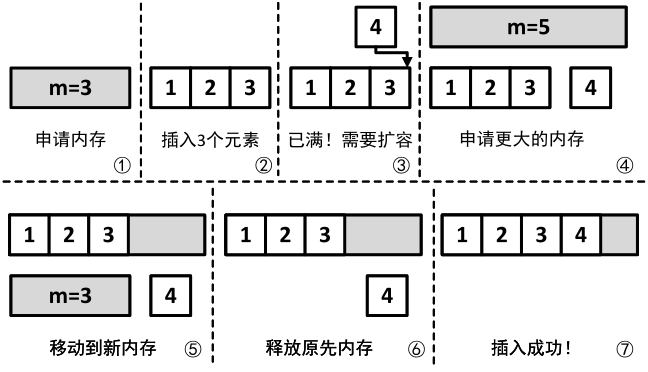
\includegraphics[width=\linewidth]{figures/vec4.pdf}
  \caption{扩容过程}
  \label{fig:vec4}
\end{figure}


可以看出,扩容是一项成本很高的操作,因为它需要开辟一块新的内存。设扩容之后的容量为$m$,则扩容算法的时间复杂度为$\Theta(m)$。由于$m$可能会很大,我们不希望经常扩容。在下一节里将会讨论一些扩容策略。

我们设计了一个方法\lstinline{resize}用来改变规模,当规模超过容量(装填因子超过1)的时候调用\lstinline{reserve}扩容。需要注意的是,一些其他的方法也会改变规模,比如插入方法\lstinline{insert}会让规模增加1,而删除方法\lstinline{remove}会让规模减1。我们需要在实现插入方法的时候也考虑扩容问题;\textit{如果您实现了缩容,那么在实现删除方法的时候也需要考虑缩容问题}。

\begin{lstlisting}
void resize(size_t n) {
    if (n > m_capacity) {
        reserve(n);
    }
    m_size = n;
}
\end{lstlisting}

\subsection{扩容策略*}
当我们调用\lstinline{resize}的时候,可以立刻知道,需要扩大到多少容量才能容纳目标的规模。但实际情况下,很多时候元素是被一个一个加入到向量中的,这个时候,按照\lstinline{resize}的策略,每次都扩容到新的规模,是一个糟糕的选择。假设初始化为了一个规模为$n$的向量,然后元素一个一个被加入,那么按照$n\to n+1 \to n+2 \to \dots$的次序扩容,每加入一个元素,都会造成至少$n$个元素的复制,时间效率极差。

因此,在面对持续插入的时候,我们需要设计新的扩容策略,以降低扩容发生的频率。这个策略应该是由向量的设计者提供的,而不是用户:如果用户知道更加合适的策略,他们会主动使用\lstinline{reserve}进行扩容。但是,用户通常没有精力用在这种细节上;这个时候,向量的设计者提供的扩容策略就会成为一个不错的备选项。

现在我们尝试为扩容策略的问题添加一个抽象的描述。当我们讨论扩容的时候,显然不需要知道向量中的数据内容是什么。因此,扩容策略作为一个算法,输入向量的当前规模$n$和当前容量$m$,输出新的容量$m'$。\textit{这个描述具有良好的可重用性,它同样可以用于缩容。}

\begin{lstlisting}
class AbstractVectorAllocator : public Algorithm<size_t(size_t, size_t)> {
protected:
    virtual size_t expand(size_t capacity, size_t size) const = 0;
    virtual size_t shrink(size_t capacity, size_t size) const = 0;
public:
    size_t operator()(size_t capacity, size_t size) override {
        if (capacity <= size) {
            return expand(capacity, size);
        } else {
            return shrink(capacity, size);
        }
    }
};
\end{lstlisting}

基于上述的分析,我们可以用这个类表示扩容策略。在后面的章节,将继承这个类并重写\lstinline{expand}方法,实现不同策略的扩容,而缩容方法则直接返回\lstinline{capacity}(永不缩容)。当您需要实现缩容的时候,也可以使用这个模板,重写\lstinline{shrink}方法。\textit{如果您对如何扩容有一些自己的想法,笔者建议您先实现自己的扩容策略,然后再阅读后面的理论部分。}

\subsection{等差扩容和等比扩容*}
\label{sec:等差和等比}
那么,应该如何设计扩容策略呢?一个简单的想法是,既然每次容量$+1$不行,那就加多一点。这种思路可以被概括为\textit{等差数列}扩容方法。如果选取$d$作为公差,那么在本节开始的那个例子中,将按照$n\to n+d \to n+2d \to \dots$的次序扩容。

\begin{lstlisting}
template <size_t D> requires (D > 0)
class VectorAllocatorAP : public AbstractVectorAllocator {
protected:
    size_t expand(size_t capacity, size_t size) const override {
        return capacity + D;
    }
};
\end{lstlisting}

这里使用了C++20引入的\lstinline{requires}语法,要求用户给定的模板参数$D>0$。因为很明显,如果$D\le 0$,\lstinline{expand}将永远扩不起来。

既然有了等差数列,另一个很容易想到的方法是按照\textit{等比数列}扩容。如果选取$q$作为公比,则会按照$n\to qn \to q^2n \to \dots$的次序扩容。

\begin{lstlisting}
template <typename Q> requires (Q::num > Q::den)
class VectorAllocatorGP : public AbstractVectorAllocator {
protected:
    size_t expand(size_t capacity, size_t size) const override {
        size_t newCapacity { capacity * Q::num / Q::den };
        return std::max(newCapacity, capacity + 1);
    }
};
\end{lstlisting}

这里允许了C++11提供的编译期有理数\lstinline{std::ratio}作为模板参数,\lstinline{Q::num}表示分子,而\lstinline{Q::den}表示分母。请注意,需要保证新的容量比原有容量大,否则扩容就没有意义。上面的做法保证了容量至少会扩大1。比如,当$Q=\frac{3}{2}$,往容量为0的向量里连续插入元素时,容量变化为$0\to 1\to 2\to 3\to 4\to 6\to 9\to \dots$,如果没有容量至少扩大1的设计,等比扩容将永远停留在0容量。

\subsection{分摊复杂度分析*}
\label{vec:分摊复杂度分析}
很显然,进行单次扩容操作的时候,等差扩容的时间复杂度为$O(n+d) = O(n)$,等比扩容的时间复杂度为$O(qn) = O(n)$(因为$q$是常数),两者看起来没有区别;甚至和我们已经知道效率很低的情况($d=1$的等差扩容)也没有区别。这也意味着,我们评价时间效率的方法可能出现了一些问题。

问题的关键在于,我们设计扩容策略的目的是按照等差或等比的\textit{数列}扩容,而不是\textit{一次}扩容。所以,评价这两种扩容规则的标准,不是进行一次扩容的效率或进行一次扩容后的装填因子,而是比较一系列扩容操作的总体效率和在这一系列扩容操作中的平均装填因子。用已有的复杂度分析工具不足以对这两种策略的效率进行准确评价。
为了对\textit{一系列}操作进行分析,需要引入新的复杂度分析标准。

一般地,假设$O_1, O_2, \dots, O_n$是连续进行的$n$次操作,则当$n\to\infty$,这$n$次连续操作所用时间的\textit{平均值}的复杂度,称为这一操作的\textbf{分摊复杂度},对分摊复杂度的分析称为\textbf{分摊分析}。分摊分析的原则之一是:使用相同效果的操作序列。所以,要比较上述两种算法,不应该把每次操作取为“进行一次扩容”(因为两种方法扩容量不一样),而应该取为“向量$V$的规模增加$1$”。连续进行$n$次操作,就可以考虑向量$V$的规模从$0$增长为$n$的过程。

在等差扩容方法中,容量依次被扩充为$d,2d,3d,\dots,n$,共进行$\frac{n}{d}$次扩容。
因此,分摊复杂度为:
$$
T(n) = \frac{d + 2d + 3d + \dots + n}n = \frac{\left(\frac{n}{d}\right)\cdot d + \frac{\left(\frac{n}{d}\right)\left(\frac{n}{d}-1\right)}2\cdot d}n = \frac{\frac{n}{d}+1}2 = \Theta\left(\frac nd\right)
$$

另一方面,进行$k$次扩容之后的装填因子至少为$\frac{kd}{(k+1)d}=\frac{k}{k+1}$,当$k\to\infty$时,装填因子趋于100\%。

在等比扩容方法中,容量被依次扩充为$q,q^2,q^3,\dots,n$,共进行$\log _q n$次扩容。
因此,分摊复杂度为:
$$
T(n)=\frac{q+q^2+q^3+\dots+n}n=\frac{q\cdot\frac{1-n}{1-q}}n=\Theta\left(\frac{q}{q-1}\right)=O(1)
$$

另一方面,装填因子不断在$\left[\frac 1q,1\right]$之间线性增长,平均装填因子为$\frac{1+q}{2q}$。可以看出,不管怎样选择$q$,对分摊复杂度都没有影响,而更小的$q$能够带来更大的平均装填因子。当选择$q=2$时,平均装填因子为75\%。

可以看出,等比扩容的装填因子并没有很低,而换来了分摊时间复杂度上巨大的优化。因此,我们倾向于选择等比扩容。至于等比扩容的公比,则是一个值得讨论的话题。从上面的推导中,我们发现分摊时间复杂度的系数为$\frac{q}{q-1}$,它会随$q$的增加而降低;另一方面,平均装填因子也会随$q$的增加而降低。因此,选择更大的$q$,事实上是以时间换空间的做法。

因为分摊$O(1)$已经很快,所以通常选取的$q$比较小。常见的公比选择有2和$\frac{3}{2}$。邓书上介绍的版本选择了2,这也是GCC和Clang的选择;而MSVC则采用更节约空间的$\frac{3}{2}$。

需要指出的是,等比扩容也存在一些劣势:容量越大,装填因子不高带来的空间浪费愈发明显,所以有些对空间要求较高的情况下,也采用二者相结合的方式:在容量比较小时等比扩容、在容量比较大的时候等差扩容。这种思想在《网络原理》里的\textit{慢启动}中得到了应用。

最后,既然有等比扩容,必然也有等比缩容。当我们讨论缩容的时候,通常需要结合一个\textbf{缩容阈值},当装填因子低于这个阈值时才引发缩容,而不是每当规模低于容量时就缩容,否则就丧失了向量的灵活性。尽管本书不实现缩容(相当于缩容阈值为0),但当缩容和缩容阈值被纳入讨论,可以命制一些有趣的问题。设等比扩容的公比为$q_1>1$,等比缩容的公比为$q_2 <1$,缩容阈值为$\theta$,\textit{您可以进行思考和计算,这三个变量满足什么条件时,才能保证对于任意的、由插入和删除组成的操作序列,扩容和缩容总和的分摊时间复杂度为}$O(1)$。

\section{插入、查找和删除}

对于任何数据结构,都有三种基本的操作:
\begin{enumerate}
    \item \textbf{插入}(insert):向数据结构中插入一个元素。
    \item \textbf{查找}(find):查找一个元素在数据结构中的位置。
    \item \textbf{删除}(delete):从数据结构中移除一个元素。
\end{enumerate}

在这一节中,我们以向量为例介绍这三种基本的操作。

\subsection{插入一个元素}
\label{sec:插入一个元素}
要将待插入的元素$e$插入到$V[r]$,那么可以将原来的向量$V[0$:$n]$分成$V[0$:$r]$和$V[r$:$n]$两部分。

\begin{itemize}
    \item 插入之前,向量是$V[0$:$r]$,$V[r$:$n]$。
    \item 插入之后,向量是$V[0$:$r]$,$e$,$V[r$:$n]$。
\end{itemize}


可以发现,在插入的前后,前一段$V[0$:$r]$的位置是不变的,而后一段$V[r$:$n]$需要整体向后移动1个单元的位置。据此,可以设计下面的算法,算法的原理如图\ref{fig:vec5}所示。

\begin{lstlisting}
Rank insert(Rank r, const T& e) override {
    std::move_backward(m_data.get() + r, m_data.get() + m_size, m_data.get() + m_size + 1);
    m_data[r] = e;
    ++m_size;
    return r;
}
\end{lstlisting}

这里需要使用\lstinline{std::move_backward}而不能用\lstinline{std::move},因为向后移动1个单元这个过程,需要先移动最后一个元素、再移动倒数第二个元素、以此类推;如果从第一个元素开始移动,就会覆盖掉还没移动的元素。如果您对STL算法不熟练,也可以改写为熟悉的循环形式。

\begin{figure}
  \centering
  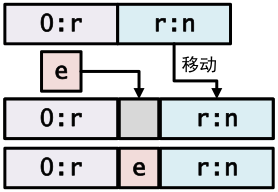
\includegraphics[width=0.4\linewidth]{figures/vec5.pdf}
  \caption{往向量中插入一个元素}
  \label{fig:vec5}
\end{figure}


在上面的算法中忽略了一点:插入有可能造成装填因子大于1的问题。如果准备插入的时候发现向量已满(装填因子等于1),那么应当先使用上一节讨论的扩容策略,扩大向量的容量,然后再执行插入。您会发现,扩容的过程中包括了一次移动,\lstinline{std::move_backward}又包括一次移动,这两次移动中会有一些重复的、不必要的赋值操作。不过,因为扩容被调用的次数很少,我们可以忽略这些额外的性能损失。

为了让我们在上一节设计的算法被嵌入到向量里来,我们可以为向量模板增加一个参数,写成下面这样的形式。

\begin{lstlisting}
template <typename T, typename Alloc = VectorAllocatorGP<std::ratio<3, 2>>>
    requires std::is_base_of_v<AbstractVectorAllocator, Alloc>
\end{lstlisting}

在上面这个模板参数表声明中,我们规定模板的第二个参数\lstinline{Alloc}必须是我们上面实现的\lstinline{AbstractVectorAllocator}的派生类。用户可以不显式地指定扩容策略,而选择我们默认的策略(公比为$\frac{3}{2}$的等比扩容)。加入这个参数之后,我们只需要在\lstinline{insert}的开头进行一次判断,就可以自动地在插入满向量时进行扩容。

最后,我们上面实现的插入算法,传入的是\lstinline{const}引用类型,这意味着元素并没有被真正的“插入”,被实际插入的是一个副本。如果我们希望让元素真正被插入,那么应当使用移动语义。移动语义版本的插入算法和复制语义基本相同。如前所述,以后将不再展示移动语义的版本。

\begin{lstlisting}
Rank insert(Rank r, T&& e) override {
    if (m_size == m_capacity) {
        reserve(Alloc {}(m_capacity, m_size));
    }
    std::move_backward(m_data.get() + r, m_data.get() + m_size, m_data.get() + m_size + 1);
    m_data[r] = std::move(e);
    ++m_size;
    return r;
}
\end{lstlisting}

\subsection{平均复杂度分析}
为了更定量地分析插入操作的时间效率,引入一个新的复杂度分析策略:\textbf{平均复杂度}。

在介绍复杂度时曾经强调,复杂度是依赖于数据\textit{规模},不依赖于输入\textit{情况}的分析手段。在上面的插入算法中,数据规模通常认为是$n$,而$r$是具体情况带来的参数。为了研究不同具体情况对算法时间效率的影响,有三种常见的分析手段:

\begin{enumerate}
    \item \textbf{最坏时间复杂度}:研究在情况最坏的情况下的复杂度。很多算法有硬性的时间限制(如在复试的机试中,通常要求输出结果的时间不能多于1s或2s),此时常常使用最坏时间复杂度分析。这是最常用的时间复杂度分析。
    \item \textbf{最好时间复杂度}:研究在情况最好的情况下的复杂度。研究最好时间复杂度的意义远小于最坏时间复杂度。最好时间复杂度有时用于嘲讽某种算法的效率:在最好的情况下,这种算法的复杂度也只能达到(某个复杂度),而我的新算法在最坏的情况下也可以达到(某个更好的复杂度)。
    \item \textbf{平均时间复杂度}:研究在平均情况下的复杂度。
如果没有硬性的时间限制,则平均时间复杂度往往能更好地反映一个算法的总体时间效率。
平均时间复杂度需要知道每种情况发生的\textit{先验}概率,在这个概率的基础上计算$T(n)$的\textit{数学期望}的复杂度。在针对现实数据的实验研究中,常见的假设包括正态分布、帕累托(Pareto)分布和泊松(Poisson)分布;而在《数据结构》学科中,通常假设成\textit{等可能的分布},以方便进行理论计算。
\end{enumerate}

平均复杂度很容易和分摊复杂度发生混淆,需要加以区分。下面是它们的一些典型的差异:
\begin{enumerate}
    \item 分摊复杂度是\textit{一系列}连续操作的\textit{平均}效率,而平均复杂度是\textit{单次}操作的\textit{期望}效率。
    \item 分摊复杂度的一系列连续操作是有可能(通常都)存在后效的,而平均复杂度只讨论单次操作的可能情况。
    \item 分摊复杂度需要指定每次进行何种的\textit{基本操作},而平均复杂度需要指定各种情况的\textit{先验概率}。
\end{enumerate}

最坏、最好、平均时间复杂度对应统计里的\textit{最大值}、\textit{最小值}和\textit{数学期望}。显然,其他统计量,比如\textit{方差},在分析的时候也是有价值的,也深得科研人员重视。但在《数据结构》的考试中,是不会涉及到这些统计量的分析的,只需要知道最坏、最好和平均时间复杂度的分析技术即可。

现在回到插入的算法,它的时间复杂度是$\Theta(n-r)$。显然,最好时间复杂度是$O(1)$(插入在末尾的情况),最坏时间复杂度是$\Theta(n)$(插入在开头的情况)。这里有略微不严谨的地方,因为$r$的最大值可以取到$n$,此时$n-r=0$,不再符合复杂度记号的定义;不过,因为我们清楚任何算法的时间都不可能为0,所以一般不在这个细节上做区分。

为了求平均时间复杂度,一个合理的假设是,$r$的取值对于$[0$:$n+1]$之间的整数是等概率的(注意有$n$个可以插入的位置,而不是$n-1$个)。在这个假设下,容易算出单次插入的平均时间复杂度为$\Theta(n)$。

\subsection{查找一个元素}
\label{seg:查找一个元素}
查找需要返回找到的位置。
对向量而言,只需要得到被查找元素的\textit{秩}就可以了。
和插入、删除相比,查找具有更加丰富的灵活性,甚至于一些编程语言(如SQL)的核心就是查找。

最简单的查找是\textit{按值查找}。即,给定被查找元素的值,在数据结构中找到等于这个值的元素。对于更加复杂的查找类型,比如\textit{按区间查找}等,人们设计了更加复杂的数据结构来应对。对于按值查找的问题,最简单的方案就是检测向量中的每个元素是否等于要查找的元素$e$,如果等于,就把它的秩返回。

\begin{lstlisting}
Rank find(const T& e) const override {
    for (size_t i { 0 }; i < m_size; ++i) {
        if (m_data[i] == e) {
            return i;
        }
    }
    return m_size;
}
\end{lstlisting}

关于找不到的情况,有多种处理方式。上面采用的方法是返回无效的秩,除了返回序列尾部溢出的\lstinline{m_size}之外,返回序列头部溢出的$-1$也是常见的选择。此外,也可以将返回值的类型改为\lstinline{std::optional},当找不到的时候返回一个无效值。

设$e$在向量中的秩为$r$,那么在\textit{查找成功}的情况下,上述算法的时间复杂度为$\Theta(r)$。在\textit{查找失败}的情况下,算法的时间复杂度为$\Theta(n)$。这里可以分析,在等可能条件下,查找成功时的平均时间复杂度是$\Theta(n)$。
注意,查找成功的概率是一个很难假设的值,所以在分析平均时间复杂度时,通常只分析“查找成功时”和“查找失败时”的平均时间复杂度,而不会将它们混为一谈。

因为对于向量$V$和待查找元素$e$的情况没有更多的先验信息,所以暂时也没有比上面更高效的解决方案。
\textbf{利用信息思考}是计算机领域重要的思维方式。在设计算法时,应尽可能利用更多的先验信息。反之,如果先验信息不足,则算法的效率受到信息论限制,不可能会特别高。这个思维方式在后文介绍各种算法的设计过程时,还会反复出现。

不过,这个算法还是有一些值得推敲的地方:如果$e$在向量$V$中出现了多次,那么这个算法只会返回\textit{最小}的秩。\textit{您可以思考一下,如何将其修改成返回最大的秩?并分析修改后的算法时间复杂度变化。}

\subsection{删除一个元素}
\label{seg:删除一个元素}
删除元素是插入元素的逆操作。在插入元素时,让被插入元素的后继\textit{后移};因此在删除元素的时候,只需要让被删除元素的后继\textit{前移}即可。需要注意前移和后移在方向上的差别,插入时的\lstinline{std::move_backward},逆操作应该是\lstinline{std::move}。

\begin{lstlisting}
T remove(Rank r) override {
    T e { std::move(m_data[r]) };
    std::move(m_data.get() + r + 1, m_data.get() + m_size, m_data.get() + r);
    --m_size;
    return e;
}
\end{lstlisting}

和插入一样,可以分析出删除操作时间复杂度$\Theta(n-r)$,平均时间复杂度$\Theta(n)$,空间复杂度$O(1)$。到此为止,我们实现了完整的\lstinline{Vector}类,可以开始实验了。如果您自己完成了向量的设计,可以使用\textit{VectorTest.cpp}进行简单的功能测试,并在实验中将\lstinline{dslab::Vector}替换为自己的向量类。

\subsection{实验:插入连续元素}

在这个实验中,我们将用实验观察,等差扩容和等比扩容的时间效率差异。因为我们评估的是分摊时间,所以需要构造一个插入连续元素的场景来进行观察。从\ref{sec:插入一个元素}节中我们知道,在位置$r$插入一个元素的时间复杂度为$\Theta(n-r)$。为了降低插入连续元素这个操作本身对,更好地观察扩容时间,我们固定每次都在向量的末尾插入元素。代码可以在\textit{VectorInsert.cpp}中找到。

我们构造下面的类,作为插入连续元素问题的基类。因为在测试过程中,每次连续插入结束之后,需要将向量重置为空(避免已分配的空间影响),所以这里定义了一个\lstinline{reset}方法。

\begin{lstlisting}
class VectorInsertProblem : public Algorithm<size_t(size_t)> {
public:
    virtual void reset() = 0;
};
\end{lstlisting}

返回值定义为连续插入结束后的向量容量,因为笔者希望观察连续插入结束之后扩容到了多大。您也可以将其改为\lstinline{void}或者其他您希望观察的变量。接下来,我们让在\ref{sec:等差和等比}节中定义的等差扩容和等比扩容策略,作为\lstinline{Vector}类的参数传入。

\begin{lstlisting}
template <typename Vec>
    requires is_base_of_v<AbstractVector<size_t>, Vec>
class VectorInsertBasic : public VectorInsertProblem {
    Vec V;
public:
    size_t operator()(size_t n) override {
        for (size_t i { 0 }; i < n; ++i) {
            V.insert(V.size(), i);
        }
        return V.capacity();
    }
    void reset() override {
        V.clear();
    }
};
\end{lstlisting}

上面的模板接受一个\lstinline{Vec}作为向量类型名,这是为了兼容您自己写的向量类。它用到了零初始化、赋值、插入、获取容量和规模的方法,如果您继承了\lstinline{AbstractVector},这些方法都应当已经实现。您也可以创建自己的测试类参与对比测试。对于本书的示例\lstinline{Vector}实现,使用下面的模板。

\begin{lstlisting}
template <typename Alloc>
    requires is_base_of_v<AbstractVectorAllocator, Alloc>
class VectorInsert : public VectorInsertBasic<Vector<int, Alloc>> {
public:
    string type_name() const override {
        return Alloc {}.type_name();
    }
};
\end{lstlisting}

这里重载了\lstinline{type_name},否则由于模板复杂,输出的类型名会非常长。在实验的示例代码中,我们比较了$d=64$、$d=4096$、$q=\frac{3}{2}$、$q=2$、$q=4$这些情况。您可以发现,当$n$比较小的时候,差异不明显;而当$n$比较大,如达到$10^6$的量级时,$d=64$会极其缓慢,而$d=4096$也慢慢和三种等比扩容拉开距离(如果您增加一个$n=10^7$的用例,会更加明显)。相反,三种等比扩容的区别非常微小,我们可以判断出,这已经非常接近插入这些元素本身需要的时间,和扩容的关系不大。

\begin{table}
  \centering
  \caption{不同扩容方式下连续插入元素的耗时对比(单位:ms)}
  \begin{tabular}{c|ccccc}
    \toprule
       $n$ & \thead{等差 \\ $d=64$} & \thead{等差 \\ $d=4,096$} & \thead{等比\\ $q=\frac{3}2$} & \thead{等比 \\ $q=2$} & \thead{等比 \\ $q=4$} 
      \\
      % & $d=64$ & $d=4,096$ & $q=\frac{3}2$ & $q=2$ & $q=4$
    \midrule
    200,000 & 515 & 20 & 12 & 13 & 11 \\ 
    400,000 & 2318 & 57 & 22 & 21 & 21 \\
    600,000 & 3662 & 89 & 33 & 34 & 33 \\
    800,000 & 5164 & 121 & 43 & 42 & 42  \\
    1,000,000 & 6649 & 155 & 50 & 54 & 51 
      \\ 
    \bottomrule
  \end{tabular}
  \label{tab:vec1}
\end{table}

如何证明上面的判断呢?去计算连续插入中原子操作的数量(计算时间复杂度的常数)是困难、繁琐且容易出错的工作。您可以加入一个$q=10^6$的向量,它的容量会直接从1跳变到$10^6$,也就是,在$n=10^6$的情况下,它没有进行任何多余的扩容。您会发现,即使是这样,也没有和上面三种等比扩容有显著差异,从而能够验证上面的判断。这种\textit{实验}方法在计算机学科的学习中是一个有力武器。\textit{这个实验请您自己完成,您也可以加入一些自己实现的其他扩容策略来观察效果。比较有挑战性的工作是,在实现缩容之后,类似本实验,设计一个新的实验评估缩容的效果(请注意,缩容本身是时间换空间的做法,仅仅测试缩容的时间性能是不合适的)。}

需要指出的是,这个实验结果只是粗略性的,因为连续插入而不做其他事情是一个非常特殊的用例。当这种情况真正发生的时候,应当直接\lstinline{reserve}足够大的空间,而不是让向量按照设计者提供的默认扩容方案慢慢扩容。

\subsection{实验:向量合并}
\label{vec:向量合并}
如果要插入的不是单个元素,而是多个元素,情况会发生什么变化呢?现在,假设我们有两个向量$V[0$:$n]$和$V_1[0$:$n_1]$,我们希望将整个$V_1$插入到$V$的位置$r$处,实现向量合并。代码可以在\textit{VectorConcat.cpp}中找到。\textit{这个问题不难,建议您自己实现算法参与对比}。

\begin{lstlisting}
class VectorConcat : public Algorithm<Vector<int>&(Rank)> {
protected:
    Vector<int> V {}, V1 {};
public:
    void initialize(int n, int n1) {
        V.reserve(static_cast<size_t>(n) + n1);
        V1.reserve(n1);
        V.resize(n);
        V1.resize(n1);
    }
};
\end{lstlisting}

和上一节类似,我们定义了一个辅助函数用来对问题进行初始化。我们不希望扩容影响实验结果,所以预先给$V$分配了$n+n_1$的空间。

如果我们采用\ref{sec:插入一个元素}节中介绍的方法,将$V_1$中的元素一个一个插入到该位置,那么时间复杂度会高达$\Theta((n-r)\cdot n_1)$,平均$\Theta(n\cdot n_1)$,略显笨重。

\begin{lstlisting}
// VectorConcatBasic
Vector<int>& operator()(Rank r) override {
    for (int i : V1) {
        V.insert(r, i);
        ++r;
    }
    return V;
}
\end{lstlisting}

您可以敏锐地发现,只要再次使用在讨论单元素插入时的分析方法,就可以得到更加高效的算法。要将待插入的向量$V_1$插入到$V[r]$,那么可以将原来的向量$V[0$:$n]$分成$V[0$:$r]$和$V[r$:$n]$两部分。
\begin{enumerate}
    \item 插入之前,向量是$V[0$:$r]$,$V[r$:$n]$。
    \item 插入之后,向量是$V[0$:$r]$,$V_1$,$V[r$:$n]$。其中,$V[r$:$n]$被转移到了$V[r+n_1$:$n+n_1]$的位置上。
\end{enumerate}

这样设计出了一个批量插入的算法,两种方法的对比如图\ref{fig:vec6}所示。


\begin{lstlisting}
// VectorConcatFast
Vector<int>& operator()(Rank r) override {
    V.resize(V.size() + V1.size());
    move_backward(begin(V) + r, end(V) - V1.size(), end(V));
    move(begin(V1), end(V1), begin(V) + r);
    return V;
}
\end{lstlisting}


\begin{figure}
  \centering
  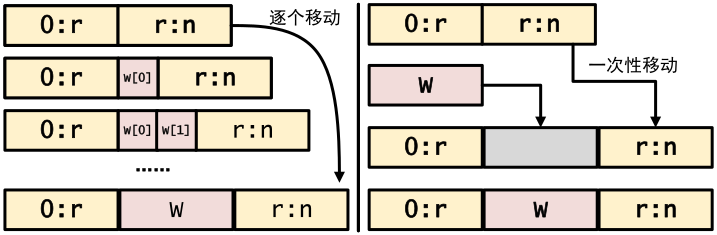
\includegraphics[width=0.9\linewidth]{figures/vec6.pdf}
  \caption{向量合并的两种方法}
  \label{fig:vec6}
\end{figure}

\textit{您可以自行分析上述批量插入算法的时间复杂度和平均时间复杂度。}因为已经预先\lstinline{reserve},这里\lstinline{resize}可以保证在$O(1)$时间里完成。
示例程序中进行了四类情况的评估:插入少量元素到开头、插入大量元素到开头、插入少量元素到结尾、插入大量元素到结尾。这里的少量可以认为是常数$n_1 = O(1)$,而大量可以认为$n_1 = \Theta(n)$。\textit{您可以对比前面得到的时间复杂度,验证您对这两个算法的评估结论。}
\textit{您也可以将上述上述两个示例程序和您自己的实现进行对比。}

\begin{table}
  \centering
  \begin{threeparttable}[c]
  \caption{向量合并算法的耗时对比(单位:ms)}
  \begin{tabular}{c|cc}
    \toprule
      \tnote{①}  & 逐个插入 & 批量插入  
      \\
    \midrule
    插入少量元素到开头 & 1\tnote{②} & 4 \\
    插入大量元素到开头 & 1060 & 7 \\
    插入少量元素到结尾 & 0 & 0 \\
    插入大量元素到结尾 & 5 & 2 \\ 
    \bottomrule
  \end{tabular}
  \begin{tablenotes}
      \item [①] $n=2\times10^5$,少量元素$=10^2$,大量元素$=10^5$。
      \item [②] 在这个场景下逐个插入反而性能更高,看起来是反直觉的,它来自于编译器优化。
    \end{tablenotes}
  \label{tab:vec2}
  \end{threeparttable}
\end{table}

批量插入的算法中体现出的\textit{用块操作代替多次单元操作}的思想,在以线性表为背景的算法设计题中应用广泛。
在我们的实现中,插入操作和扩容操作是\textit{解耦}的:容量已经被预先分配好。在实际情况下,我们也需要同时考虑扩容的成本。按照解耦的实现,在扩容申请了新的数组空间之后,会将原数组的元素复制过去,然后再执行插入,对这些元素进行移动。很显然,$V[r]$之后的元素被移动了两次。事实上,如果进行耦合的实现,可以让这些元素只被移动一次:在扩容申请了新的数组空间之后,$V[r]$之后的元素可以直接移动到它们的目的位置,为$V_1$里的元素“空出一块空间”。\textit{您可以自己实现这个耦合算法。因为需要在外部访问\lstinline{Vector}里的成员,因此您应当将您的类或函数生声明为友元。}

\subsection{实验:按值删除元素}
\label{sec:按值删除元素}
在\ref{seg:删除一个元素}节,我们讨论的删除是按位置删除,具体到向量就是按\textit{秩}删除。另一种删除的方式是按\textit{值}删除,也就是说,我们给定一个元素$e$,想要删除向量中和$e$相等的每一个元素。代码可以在\textit{VectorRemove.cpp}中找到。\textit{同样,建议您自己实现一个算法。}

在分析这个问题之前,先对\textit{按值}操作进行一些深层次的理解。我们知道,数据结构是元素的集合,元素之间是互不\textit{相同}的,但这并不妨碍它们\textit{相等},因为我们可以定义“相等”(反映到C++中,就是重载运算符\lstinline{operator==})。比如说,我们定义值相同为“相等”,这样就不需要考虑元素的地址;这是按值删除的思路。顺着这个思路,我们可以扩展按值删除到更加一般的按\textit{条件}删除。比如说,向量里的元素是一个结构体,我们定义结构体的某个属性相同为“相等”,而其他属性可以不被考虑;此时,某个属性等于给定的值就是我们定义的\textit{条件}。在C++的STL中,按值删除对应的算法是\lstinline{std::remove},而按条件删除对应的算法是\lstinline{std::remove_if},二者具有高度的相似性。其他的一些算法也有相应的“按条件”版本,您可以根据需要自行了解,这里不再赘述。

下面我们来讨论按值删除元素的问题。为了评估算法的性能,示例程序构造了一个场景:在一个规模为$n$的向量中,第奇数个元素为1,第偶数个元素为0,我们的算法将要删除所有的0,也就是说删除一半的元素。

\begin{lstlisting}
class VectorRemove : public Algorithm<size_t, int> {
protected:
    Vector<int> V {};
    virtual void batchRemove(int e) = 0;
public:
    size_t operator()(int e) override {
        size_t n = V.size();
        batchRemove(e);
        return n - V.size();
    }
    void initialize(size_t n) {
        V.resize(n);
        for (size_t i { 0 }; i < n; ++i) {
            V[i] = i % 2;
        }
    }
};
\end{lstlisting}

和上一节一样,我们从最朴素的想法开始:逐个查找、逐个删除。我们在向量$V$中查找要删除的$e$,每发现一个就删除一个,直到没有等于$e$的元素为止。如图\ref{fig:vec7}所示。

\begin{lstlisting}
// VectorRemoveBasic
void batchRemove(int e) override {
    Rank r { 0 };
    while (r = find(begin(V), end(V), e) - begin(V), r < V.size()) {
        V.remove(r);
    }
}
\end{lstlisting}

\begin{figure}
  \centering
  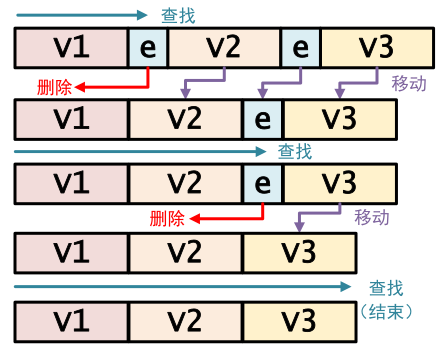
\includegraphics[width=0.6\linewidth]{figures/vec7.pdf}
  \caption{向量按值删除元素:逐个查找、逐个删除}
  \label{fig:vec7}
\end{figure}

上述朴素算法的空间复杂度是$O(1)$,但是时间效率是很低的。这里使用的\lstinline{std::find},原理和\ref{seg:查找一个元素}节介绍的查找一样,时间复杂度为$\Theta(r)$。\lstinline{std::find}返回的是一个迭代器,和起始迭代器\lstinline{std::begin}相减之后就可以得到找到的位置(秩)。而另一方面,在找到之后,\lstinline{remove}的时间复杂度为$\Theta(n-r)$。所以,每次循环的时间复杂度为$\Theta(n)$。在极端情况下(比如我们设计的实验场景),有$\Theta(n)$个元素要被删除,此时时间复杂度为$\Theta(n^2)$。\textit{考虑到C++的标准算法库在考试中手写代码时通常不能使用(阅卷者可能看不懂),所以如果您不熟练,非常建议您在理解这些标准算法之后把它改写成C语言的风格,直到您能熟练地在STL和C语言风格之间做转换为止。学习的时候使用STL的好处是精简代码,减少记忆量,容易抓住主要矛盾。}

在设计算法的时候,题目不一定会给出要求的复杂度。这个时候,可以对比一下\textit{相似问题}的复杂度。比如,之前介绍讨论批量插入(向量合并)的时候可以做到线性的时间复杂度,没有理由批量删除(按值删除)需要平方级的时间复杂度。因此,我们需要寻找提高时间效率的切入口。

为了降低时间复杂度,就要设法降低在算法中进行的\textit{不必要工作}。在不必要工作中,有几种比较典型。一种是\textit{不到位工作},它代表了在算法中,本能够一步到位的计算被拆分成了若干个碎片化的步骤,而产生的时间浪费。比如在向量合并的逐个插入算法中,后缀$V[r+1$:$n]$就接连移动了$n_1$次;我们通过合并这些移动实现了算法优化。

另一种是\textit{重复工作},它代表了在算法中,重复计算了同一算式造成的时间效率浪费。在上面的朴素的按值删除算法中,就有一项非常明显的重复工作。如图\ref{fig:vec7}所示,第一次检索了第一段$V_1$,第二次检索了$V_1+V_2$,第三次检索了$V_1+V_2+V_3$;这里$V_1$被检索了3次,$V_2$被检索了2次,而事实上只需要检索一次即可。在我们查找完毕的时候,可以记录下当前查找到的位置;下一次查找的时候从记录下的位置开始记录,如图\ref{fig:vec8}所示。借用C++的STL,我们对朴素算法做很小的改动就可以做到这一点,您可以对比两张图和两份代码。

\begin{lstlisting}
// VectorRemoveImproved
void batchRemove(int e) override {
    Rank r { 0 };
    while (r = find(begin(V) + r, end(V), e) - begin(V), r < V.size()) {
        V.remove(r);
    }
}
\end{lstlisting}

\begin{figure}
  \centering
  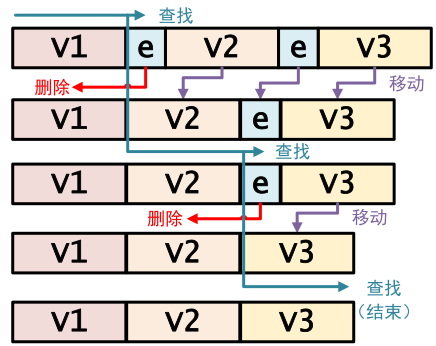
\includegraphics[width=0.6\linewidth]{figures/vec8.pdf}
  \caption{向量按值删除元素:一次查找、逐个删除}
  \label{fig:vec8}
\end{figure}

然而您会发现,在最坏的情况下(所有元素都要被删除),光是\lstinline{remove}就要花费$\Theta(n^2)$的时间,上面这个算法的优化程度仍然不够。因此,下一步优化就要从\lstinline{remove}入手,需要将\lstinline{remove}的工作展开来,看看其中哪些是不必要的。

在\lstinline{remove}中,主要消耗时间的是\textit{元素移动}的操作。您可以发现,如果$V[0$:$i]$中有$k$个元素要删除,那么最后一个元素$V[i-1]$就要向前移动$k$次:依次移动到$V[i-2]\to V[i-3]\to \dots\to V[i-k-1]$的位置上。比如,在图\ref{fig:vec8}中,$V_3$就移动了2次。
您可以敏锐地发现者正是前面所讲述的\textit{不到位工作}。这一系列的移动被拆成了$k$次,而实际上是可以一步到位,直接从$V[i-1]$移动到目标位置$V[i-k-1]$的。

为什么可以直接移动到目标位置呢?注意到,无论是上面的Basic还是Improved算法,当检索到$V[i]$的时候,前缀$V[0$:$i]$的所有元素都已经被检索过了,因此$k$的值已经确定了,并且前$i-1$个元素已经移动到了正确的目标位置。所以您可以用归纳法的思路,证明直接移动的正确性。证明完成之后,剩下的就只有编码的工作了。\textit{强烈建议您自己完成这个算法再阅读示例程序。}下面展示了一种实现。

\begin{lstlisting}
// VectorRemoveFSP
void batchRemove(int e) override {
    Rank k { 0 };
    for (Rank r { 0 }; r < V.size(); ++r) {
        if (V[r] == e) {
            ++k;
        } else {
            V[r - k] = move(V[r]);
        }
    }
    V.resize(V.size() - k);
}
\end{lstlisting}

非常显然,现在时间复杂度被缩减到$\Theta(n)$了。上面这个算法的思路可以被概括为\textit{快慢指针},这是线性表算法设计中非常典型的技巧。快指针即探测指针,指向$V[r]$;慢指针即更新指针,指向$V[r-k]$。快指针找到需要保留的元素,然后将它们移动到慢指针的位置处。如图\ref{fig:vec9}所示。

\begin{figure}
  \centering
  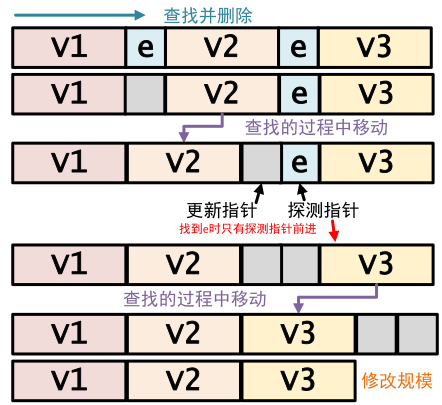
\includegraphics[width=0.6\linewidth]{figures/vec9.pdf}
  \caption{向量按值删除元素:快慢指针}
  \label{fig:vec9}
\end{figure}

\begin{table}
  \centering
  \caption{按值删除算法的耗时对比(单位:ms)}
  \begin{tabular}{c|ccc}
    \toprule
       $n$ & Basic & Improved & 快慢指针  
      \\
    \midrule
    $10^3$ & 2 & 0 & 0 \\
    $10^4$ & 213 & 19 & 0 \\
    $10^5$ & 20192 &  1972 & 1
      \\ 
    \bottomrule
  \end{tabular}
  \label{tab:vec3}
\end{table}

您可以通过示例程序的测试明显感知到这三种算法的性能差异。作为结束,上述算法在C++的STL中有一个简单的记法:

\begin{lstlisting}
// VectorRemoveErase
void batchRemove(int e) override {
    V.resize(remove(begin(V), end(V), e) - begin(V));
}
\end{lstlisting}

这里使用了STL提供的\lstinline{std::remove},它并不会真正地将$e$删除,而是将非$e$的元素都移动到向量的前半部分,并返回新的尾部迭代器。用户还需要进行一次\lstinline{resize}才能真正清除掉已经无效的后半部分,这个真正清除的过程被称为\textbf{擦除}(erase);这个方法也被称为“删除-擦除”法。STL中的向量容器\lstinline{std::vector}提供了原生的\lstinline{erase}方法,您可以直接使用它进行按值删除。

\section{置乱和排序}
一般数据结构重点讨论的只有插入、删除和查找三种基本操作,但向量作为一种非常基础的数据结构,经常被用来在考试中作为算法设计题的背景。下面这两个小节分别从\textit{熵增}和\textit{熵减}的角度出发,讨论\textbf{置乱}(shuffle)和\textbf{排序}(sort)的算法。

\subsection{实验:随机置乱*}
通常说的置乱都是指随机置乱。给定一个向量$V$和一个随机数发生器\lstinline{rand},随机打乱向量中的元素。在理论分析的时候,可认为随机数发生器是\textit{理想的},即每次调用能够随机生成一个\textit{非负整数}。当然现实中的随机数发生器做不到理想,我们将在本小节的末尾讨论它们的区别。

置乱算法接收一个向量将它置乱。代码可以在\textit{Shuffle.cpp}中找到。\textit{如果您想到了解决方案,可以先自己实现它。}

\begin{lstlisting}
class Shuffle : public Algorithm<void(Vector<int>&)> {};
\end{lstlisting}

直接看这个“向量置乱”的问题,很容易没有头绪。不妨将这个问题迁移到比较熟悉的领域:比如洗牌。
想必大家都非常熟悉洗牌。随机置乱的目的和洗牌是一样的,但如果用洗牌的方法去做随机置乱,即抽出一沓牌、把这沓牌放到牌堆底部、再抽一沓牌,则会面临三个问题:
\begin{enumerate}
    \item 您不知道重复多少次抽牌比较合理。
    \item 在有限次抽牌之后,牌的$n!$种随机次序并不是等概率的。
    \item 每次抽牌都要伴随大量的元素移动,时间效率非常低下。
\end{enumerate}

解决随机置乱问题可以从上面的第二个问题,也就是“随机次序等概率”入手。为了保证随机次序是等概率的,那么就要构造$n!$种等可能的情况。根据乘法原理,可以很自然地想到,如果将每种次序表示为一个$n$元随机变量组$(X_1, X_2, ..., X_n)$,其中$X_i$两两独立,并且$X_i$恰好有$i$个等可能的取值,那么这$n!$种次序就是等可能的了。接下来,只需要建立在全排列和这样的$n$元组的一一对应的映射关系即可。当然,不能直接把全排列用上。全排列的两个元素不是相互独立的,它自身不是符合条件的$n$元组。

为了构造符合条件的映射,又可以采用递归的思想方法:

\begin{enumerate}
    \item 如果$n = 1$,全排列和$n$元组可以直接对应。
    \item 对于$n > 1$,考虑$V[n-1]$在打乱后的秩,显然,它可以取$0,1,\dots,n-1$这$n$个等可能的值,令这个数为$X_n$,然后将$V[n-1]$从打乱前后的向量中都删除,就化为了$n-1$的情况。反复利用这个化归方法,最终可化归到$n = 1$的情况。
\end{enumerate}

以上就成功构造出了满足条件的一一映射关系,\textit{您可以在理解它的基础上自己设计相应的随机置乱算法}。下面给出了一个示例实现。

\begin{lstlisting}
void operator()(Vector<int>& V) override {
    for (auto i { V.size() }; i > 1; --i) {
        auto j { rand() % i };
        swap(V[i - 1], V[j]);
    }
}
\end{lstlisting}

显然上面这个算法是时间$\Theta(n)$、空间$O(1)$的。并且上面的分析表明,如果\lstinline{rand}真的能随机生成一个非负整数(不是随机生成一个\lstinline{unsigned int}!),那么这个算法就能将所有的$n!$个排列等概率地输出。
此外,C++11在STL中也提供了置乱算法,需要包含\lstinline{<random>}库使用。

\begin{lstlisting}
class ShuffleStd : public Shuffle {
    default_random_engine m_engine { random_device {}() };
public:
    void operator()(Vector<int>& V) override {
        shuffle(begin(V), end(V), m_engine);
    }
};
\end{lstlisting}

这里的默认随机数引擎可以被替换为其他用户定义的引擎,关于随机数引擎的问题和数据结构无关,不再赘述。默认的随机数引擎基于梅森旋转算法,产生随机数的速度较慢,但具有较好的均匀性。图\ref{fig:vec15}展示了4个元素随机置乱$10^6$次的结果,全部的24种可能情况出现的频率非常接近,平均相对误差只有大约0.4\%。

\begin{figure}
  \centering
  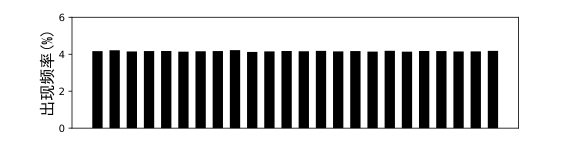
\includegraphics[width=0.7\linewidth]{figures/vec15.pdf}
  \caption{随机置乱的结果}
  \label{fig:vec15}
\end{figure}

下面回到随机生成器的问题上来,真实的\lstinline{rand}会受到位宽的限制。
如果每次随机生成一个随机的32位非负整数,那么$n$次随机一共只有$2^{32n}=o(n!)$种可能的取值,所以在$n$充分大的时候,必然会有一些排列不可能被输出。

另一方面,即使忽略位宽的限制,也不可能做到等概率输出。因为当随机数生成器的返回值是在$[0,2^k-1]$中随机生成的非负整数时,$n!$在$n\ge 3$时不是$2^k$的因子(不论$k$有多大),所以这$n!$个排列不可能是等概率的。不过,当$n$比较小时概率可以认为\textit{近似}相等,您可以在示例程序的运行结果中看出这一点。

除此之外,现实中的\lstinline{rand}是\textit{伪随机}。对于同一个种子,生成的伪随机序列是相同的,所以并不能真正“随机”地打乱向量中的元素。当然,这是另一个话题了。当我们在后面的章节讨论散列的时候,再对伪随机问题进一步探讨。

\subsection{偏序和全序*}
\label{sec:偏序和全序}
在讨论完置乱问题之后,接下来讨论排序问题。在具体介绍排序算法前,首先需要界定清除,\textbf{序}(order)是一个什么东西。在上一章定义过\textit{良序}的概念,但要对一个向量做排序,并不一定要要求它的元素是某个定义了良序关系的类型。比如说,$n$个实数同样可以关于熟知的“$\le$”排序。
因此,需要引入条件更松的序关系的定义。

将良序关系定义中的第4个条件(最小值)去掉,就变成了\textbf{全序}(total order)关系。
如果集合$S$上的一个关系$\preceq$满足:
\begin{enumerate}
    \item \textbf{完全性}。$x \preceq y $和 $y \preceq x$至少有一个成立。
    \item \textbf{传递性}。如果$x \preceq y$且$y \preceq z$,那么$x\preceq z$。
    \item \textbf{反对称性}。如果$x\preceq y$和$y\preceq x$均成立,那么$x=y$。
\end{enumerate}

那么称$\preceq$是$S$上的一个\textbf{全序关系}。显然良序关系是全序关系的子集。

和良序关系相比,全序关系更加符合常规的认知。比如,实数集上熟知的“$\le$”就是全序关系。由于\textit{完全性}的存在,凡是具有全序关系的数据类型,都可以进行排序;反之,在《数据结构》里的“通常意义的排序”问题中,都假定数据结构中的元素数据类型具有“先验的全序关系”。

在C++中,排序函数\lstinline{std::sort}接受三个参数,其中第三个参数就表示“自定义的全序关系”。基本数据类型(如\lstinline{int}和\lstinline{double}),以及一些组合类型(如\lstinline{std::tuple})定义了内置的全序关系(即熟知的“$\le$”),但也可以使用其他的全序关系进行排序。其他编程语言中的排序函数也有类似的设计。

除了全序关系之外,还有一种序关系在《数据结构》中也经常会提到:\textbf{偏序}(partial order)关系。

如果集合$S$上的一个关系$\preceq$满足:
\begin{enumerate}
    \item \textbf{自反性}。$x \preceq x $。
    \item \textbf{传递性}。如果$x \preceq y$且$y \preceq z$,那么$x\preceq z$。
    \item \textbf{反对称性}。如果$x\preceq y$和$y\preceq x$均成立,那么$x=y$。
\end{enumerate}

那么称$\preceq$是$S$上的一个\textbf{偏序关系}。偏序关系和全序关系相比,第1个条件(完全性)变成了更简单的自反性;也就是说,并不是$S$中的任意两个元素都能进行比较。比如,令$S$为“考生组成的集合”,$\preceq$定义为“考生$x$的\textit{每一门}分数都小于等于考生$y$”。您可以轻易验证,这个关系是偏序关系但不是全序关系。

在计算机编程中直接定义偏序关系是不方便的,因为$\preceq$的返回值往往是\lstinline{bool}类型,不存在\lstinline{true}和\lstinline{false}之外的第三个选项(\textit{无法比较})。并且,无法比较的情况不能随意地返回一个\lstinline{true}或\lstinline{false}的值,因为这可能导致传递性被破坏。
所以,当在编程时需要定义一个偏序关系时,往往会将它扩展成一个全序关系。比如,给$S$中的所有元素做标号,当已有的偏序关系无法比较时,则根据标号的大小进行比较。扩展成全序关系之后,就可以进行排序了。由扩展成的全序关系的不同,可能会产生不同的排序结果。

在C++20中定义了各种序关系,用于作为航天飞机运算符\lstinline{operator<=>}的返回值。比如,偏序关系被定义为\lstinline{std::partial_ordering},这个类型包括大于、小于、等价以及无法比较四种比较结果。除此之外,还提供了包括大于、小于和等于的强序关系\lstinline{std::strong_ordering}和包括大于、小于和等价的弱序关系\lstinline{std::weak_ordering}。
这两者的区别在于“等于”和“等价”,或者说“相同”和“相等”。强序关系不允许两个不同的元素相等(这是非常强的条件),而弱序关系允许。一般而言,全序关系即对应强序关系,而经过一个映射的全序关系(如二维坐标只比较一个维度) 则对应弱序关系。

\subsection{自上而下的归并排序}
\label{sec:归并排序}
现在回到向量排序的问题。
对于一个线性表,如果它的数据类型是全序的;且对其中的任意一个元素$x$,和$x$的\textit{后缀}中的任意一个元素$y$,总是有$x\preceq y$,则称它是\textbf{有序的}(ordered)。对于无序线性表,通过移动元素位置使其变为有序的过程,称为\textbf{排序}(sort)。在计算机领域所说的有序,一般都是指\textit{升序}。所以在上面的定义中使用的是\textit{后缀}。如果您想要讨论降序或者其他的顺序(比如按最小素因子排序),只需要重新定义全序关系$\preceq$,即可以回归为升序的情况进行处理。

\begin{lstlisting}
template <typename T, template<typename> typename Linear>
    requires std::is_base_of_v<AbstractLinearList<T, typename Linear<T>::position_type>, Linear<T>>
class AbstractSort : public Algorithm<void(Linear<T>&)> {
protected:
    std::function<bool(const T&, const T&)> cmp { std::less<T>() };
    virtual void sort(Linear<T>& L) = 0;
public:
    template <typename Comparator>
    void operator()(Linear<T>& L, Comparator cmp) {
        this->cmp = cmp;
        sort(L);
    }
    void operator()(Linear<T>& L) override {
        sort(L);
    }
};
\end{lstlisting}

在上面的程序中,我们规定了一个排序的抽象模板类,它接收一个线性表(通过概念限制)对其进行排序。因为排序的结果一定是一个序列,所以我们只考虑线性表。约定俗成地,我们通常使用严格的序关系,比如$<$,而不是不严格的$\le$。C++提供了模板\lstinline{std::less}来表示使用类型\lstinline{T}定义的小于运算符,用户也可以自定义仿函数传入这个模板中。

排序是计算机领域最重要的算法之一。在计算机出现至今,人们提出了各种各样的排序算法,并且仍然有不少研究者在从事着排序算法的研究。在《数据结构》中,将专门有一章讨论各种排序算法。在本节,先介绍一种最基本、最经典的排序方法:\textbf{归并排序}(merge sort)~\cite{knuth1997art}。归并排序的发明人是大名鼎鼎的冯·诺依曼(von Neumann),这位“计算机之父”在1945年设计并实现了该算法。


\begin{figure}[H]
  \centering
  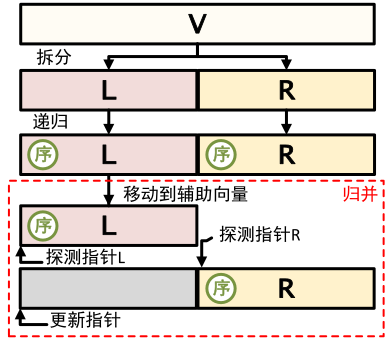
\includegraphics[width=0.5\linewidth]{figures/vec10.pdf}
  \caption{向量的归并排序}
  \label{fig:vec10}
\end{figure}


归并排序的设计采用的仍然是递归的思想:
\begin{enumerate}
    \item 规模$n\le 1$的向量总是天然有序的。
    \item 对于规模$n > 1$的向量,可以将其分成前后两部分,长度分别为$\frac{n}2$和$n-\frac{n}2$(在上一章您见过这个分法),从而将规模为$n$的问题化归为两个规模较小的子问题。这些子问题可以继续递归下去直到化为$1$。解决子问题之后,$V$的前半部分和后半部分分别有序,只需要将这2个有序序列合并为1个有序序列,就可以解决原问题了。这一合并的过程就称为\textbf{归并}(merge)。
\end{enumerate}

\textit{您可以根据上面的思想,自己实现一个归并排序的算法(一个建议是,将归并的过程提取为单独的函数以提高可读性),然后和下面的示例算法进行比较。这个代码比较长。最好自己先写一份代码,因为直接读示例代码很难记住。
注意,在《数据结构》部分,代码的记忆既不是重点也没有必要。归并排序这个知识点的核心是上面的这一段文字,即归并的思想。}

下面的示例代码既可以用于向量,又可以用于后面的章节介绍的列表。

\begin{lstlisting}
template <typename T, template<typename> typename Linear>
class MergeSort : public AbstractSort<T, Linear> {
protected:
    Vector<T> W;
    using Iterator = typename Linear<T>::iterator;
    void merge(Iterator lo, Iterator mi, Iterator hi, size_t leftSize) {
        W.resize(leftSize);
        std::move(lo, mi, std::begin(W));
        auto i { std::begin(W)};
        auto j { mi }, k { lo };
        while (i != std::end(W) && j != hi) {
            if (this->cmp(*j, *i)) {
                *k++ = std::move(*j++);
            } else {
                *k++ = std::move(*i++);
            }
        }
        std::move(i, std::end(W), k);
    }
    void mergeSort(Iterator lo, Iterator hi, size_t size) {
        if (size < 2) return;
        auto mi { lo + size / 2 };
        mergeSort(lo, mi, size / 2);
        mergeSort(mi, hi, size - size / 2);
        merge(lo, mi, hi, size / 2);
    }
protected:
    void sort(Linear<T>& L) override {
        mergeSort(std::begin(L), std::end(L), L.size());
    }
};
\end{lstlisting}

C++提供了\lstinline{std::inplace_merge}函数(传入lo、mi和hi的迭代器)来进行归并,您可以用这个函数代替上述手写的\lstinline{merge}方法。
归并排序的算法中有很多细节可以挖掘,下面列出了其中的一部分。在阅读并理解上述归并排序的算法的基础上,您可以尝试回答以下问题(其中,假定比较函数\lstinline{cmp}的时间、空间复杂度都是$O(1)$的),然后再查看后面的分析。

\textit{在归并的一开始,将前半部分移动到了辅助向量中。为什么前半部分需要移动出去,而后半部分不需要?}

在归并的过程中,事实上也采用了\textit{快慢指针}的思想。快指针(探测指针)是$j$,慢指针(更新指针)是$k$。还有一个探测指针是$i$,不过它工作在辅助向量$W$上。
如果前半部分不移动的话,$i$也会工作在原向量上,它和$k$不构成快慢关系。于是,一旦后半部分比前半部分的元素小,就会把前半部分的元素覆盖掉;而对后半部分而言,除非前半部分已经全部加入到原向量中,否则$j$永远能够在$k$前面。而当前半部分全部加入之后,$i<\mathrm{mi}-\mathrm{lo}$不再成立,循环结束。

\textit{在归并的最后,我们将前半部分(此时在辅助向量里)多余的元素移动回原向量。为什么后半部分多余的元素不需要?}

后半部分的数据没有移动出去,如果前半部分的元素已经全加入到原向量了,则后半部分剩余的元素已经在它们应该在的位置上,不需要再移动了。

\textit{辅助向量$W$的长度至少是多少?并由此确定归并排序的空间复杂度。}

辅助向量$W$的长度至少为最大的$\mathrm{mi}-\mathrm{lo}$,也就是$\frac{n}2$,因此空间复杂度为$\Theta(n)$。
这里需要注意,递归产生的$\Theta(\log n)$,相比于辅助数组的$\Theta(n)$来说可以忽略;但在解答题的场合,应当书写在解题过程中表示考虑到了此种情况。

\textit{归并排序的时间复杂度是多少?如果划分的时候,左半部分不取$\frac{n}2$而是取$kn$(其中$0<k<1$),时间复杂度又会变成多少?如果取作$\max\left(\frac{n}2, C\right)$,其中$C$是一个给定的常数,那么时间复杂度又会变成多少?}

这个问题是归并排序相关的一个经典问题,考试中也可能出现。
对于原始的归并排序(\textit{折半二分}),您可以列出$T(n)=2T\left(\frac n2\right)+\Theta(n)$的方程,递降计算出$T(n)=\Theta(n\log n)$。当取$kn$(\textit{定比二分})时做法类似,时间复杂度不会变,但常数会增加,您可以自行计算。
如果左半部分的长度存在上限$C$(\textit{定长二分}),则在$n$充分大时,$T(n)=T(n-C)+T(C)+\Theta(n)=\Theta(n^2)$。
因此两部分的划分必须按比例取,而不能受到某个固定值$C$的限制。

此类问题通常可以用\textbf{主定理}(master theorem)~\cite{bentley1980general}解决。主定理是用来处理分治算法得到的递归关系式的“神兵利器”。它的证明太过复杂,这里只陈述结论。

\begin{theorem}[主定理]
设$T(n) = aT\left(\frac nb\right) + f(n)$,则:
\begin{enumerate}
    \item 若$f(n) = O\left(n^{\log _b a - \varepsilon}\right)$,其中$\varepsilon > 0$,则$T(n) = \Theta\left(n ^ {\log _b a}\right)$。
    \item 若$f(n) = \Theta\left(n^{\log _b a}\right)$,则$T(n) = \Theta\left(n ^ {\log _b a}\log n\right)$。
    \item 若$f(n) = \Omega\left(n^{\log _b a + \varepsilon}\right)$,其中$\varepsilon > 0$,且$\overline{\lim\limits_{n\to\infty}}\frac{f\left(\frac{n}b\right)}{f(n)}<1$,则$T(n) = \Theta\left(f(n)\right)$。
\end{enumerate}

\end{theorem}

\subsection{自下而上的归并排序*}
\label{sec:自下而上的归并排序}
上一节中展示的归并排序是自上而下的。这里的“自上而下”指的是,我们首先调用整个向量的归并排序$\mathrm{mergeSort}(V)$,在这个函数中递归地调用子向量的归并排序$\mathrm{mergeSort}(L)$和$\mathrm{mergeSort}(R)$。以此类推,直到“最下方”的递归实例,也就是递归边界(只有一个元素的向量)。

自上而下的归并排序是归并排序的经典实现,下面介绍一种自下而上的方法。我们分析归并函数merge的调用次序会发现,由于归并发生在递归调用之后,所以归并的次序反而是自下而上的:首先对“最下方”的子向量做归并,得到长度为2的有序子向量。一个子向量可以被归并,当且仅当它的左半和右半的子向量已经被归并完成。

\begin{figure}
  \centering
  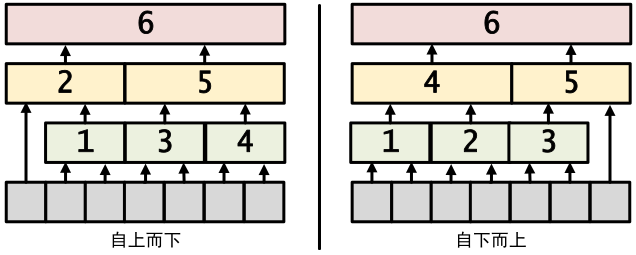
\includegraphics[width=0.8\linewidth]{figures/vec14.pdf}
  \caption{自上而下和自下而上的归并次序}
  \label{fig:vec14}
\end{figure}

如图\ref{fig:vec14}中左图所示,在自上而下的归并排序中,只要左半和右半的子向量都已经被归并完成,就会引发这两个子向量的归并。对于7个元素组成的向量,一共会触发6次归并,归并的次序在图中用1至6表示。由于一个向量的归并,只需要保证它左半和右半归并完成之后进行,而并不要求在左半和右半归并完成之后\textit{立即}进行,所以我们可以调整这6次归并的次序。我们首先将向量视作长度为1的段两两合并,然后将它视作长度为2的段(每个段内已经有序)两两合并,再视作长度为4的有序段两两合并,以此类推,直到归并整个向量为止。上面的每一步称为一\textbf{趟}(run)。这种方法同样保证了一个子向量晚于它的左半和右半被归并,因而也能保证正确性。

如图所示,因为向量规模不一定是2的幂次,每一趟的末尾处需要特殊处理。从图中还可以看出,自下而上的归并排序对于子向量的分拆方式,是有可能和自上而下不同的。
下面展示了自下而上的归并排序的一个实现,它复用了自上而下版本的merge函数,只是在调用merge的次序上和自上而下的版本有所区别。

\begin{lstlisting}
template <typename T, template<typename> typename Linear>
class MergeSortUpward : public MergeSort<T, Linear> {
protected:
    void sort(Linear<T>& L) override {
        auto n { L.size() };
        for (size_t width { 1 }; width < n; width *= 2) {
            auto lo { std::begin(L) };
            Rank i { 2 * width };
            while (i < n) {
                auto mi { lo + width };
                auto hi { mi + width };
                this->merge(lo, mi, hi, width);
                lo = hi;
                i += 2 * width;
            }
            if (n + width > i) {
                auto mi { lo + width };
                auto hi { std::end(L) };
                this->merge(lo, mi, hi, width);
            }
        }
    }
};
\end{lstlisting}

外层循环进行的次数(也就是趟数)很显然是$\lceil \log n\rceil$。在每一趟中,各个归并段是互不重叠,且可以证明至少有$\frac{2}{3}$的元素参加了归并,所以每一趟的时间复杂度为$\Theta(n)$。因此,自下而上的归并排序时间复杂度同样是$\Theta(n\log n)$。

自下而上的归并排序的时间消耗随$n$的增长是不平滑的。当$n$从$2^k$增长到$2^k+1$时,自下而上的归并排序需要增加整整一趟;因此,它在$n$略小于或等于一个2的幂次的时候表现更好,而在略大于一个2的幂次时表现较差。关于这部分性能的具体讨论,参见《排序》章中的Tim排序。

\subsection{基于比较的排序的时间复杂度}
\label{vec:基于比较的排序的时间复杂度}
归并排序是一种\textbf{基于比较}(comparison-based)的排序。
所谓基于比较,就是在算法进行过程的每一步,都依赖于元素的比较(即调用\lstinline{cmp})进行。基于比较的排序是针对\textit{全序关系}设计的。大多数的排序算法都是基于比较的。
还有一些不基于比较的排序,它们不是针对待排序数据类型的全序性设计的,而是针对待排序数据类型的其他性质设计的,因而应用范围会更小。在后文中会介绍一些不基于比较的排序。

下面将说明一个重要结论:
\begin{theorem}
基于比较的排序在最坏情况下的时间复杂度为$\Omega(n\log n)$。
\end{theorem}

这是本书中第一次使用信息论方法,讨论时间复杂度的\textit{最优性}。信息论方法在考试中通常不会直接考到,但用信息论的思路,有助于在算法设计题中判断自己是否能得到时间复杂度层面上的满分。此外,信息论方法也对记忆知识点有帮助。

\begin{enumerate}
    \item 因为是最坏情况,不妨假设所有元素互不相等。在排序算法开始之前,这$n$个元素可能的顺序关系有$n!$种,而在排序算法开始之后,这$n$个元素可能的顺序关系只有1种(因为已经找到了它们的顺序)。
    \item 另一方面,每次比较都有两种结果(\lstinline{if}分支和\lstinline{else}分支)。剩下的可能的顺序关系被分为2个部分,根据比较结果,只保留其中的1个部分。在最坏情况下,每次保留的都是元素较多的部分,从而每次比较至多排除一半的可能。
\end{enumerate}

综合以上两点,至少需要进行$\log_2(n!)=\Theta(n\log n)$次比较,于是就证明了上述的定理。最后一步的结论基于一个重要的公式:

\begin{theorem}[斯特林公式]
    在$n\to\infty$时,$n!\sim \sqrt{2\pi n}\cdot \left(\frac ne\right)^n$。
\end{theorem}

这一公式的证明是纯数学的话题。感兴趣的话可自行在网上查找,这里不再叙述。
在《数据结构》的学习中需要记住的公式并不多,斯特林(Stirling)公式是必须记住的公式之一。或者,您也可以只记住$\log(n!)=\Theta(n\log n)$,因为这是它的主要应用。

由此可见,归并排序在基于比较的排序中,已经达到了最优的时间复杂度。当然,空间复杂度不是最优的,它需要$\Theta(n)$的额外空间。关于排序的更多性质,在后面的专门章节中将继续分析。从这个时间复杂度下界也可以看出,排序需要付出的努力总是比置乱要高,这也符合我们对信息的一般认知:排序是熵减的过程,而置乱是熵增的过程,熵减总是要付出更多的努力。

\subsection{信息熵*}
\label{vec:信息熵}
基于上一小节的讨论,
本小节对香农(Shannon)提出的\textbf{信息熵}(information entropy)概念进行简要的介绍。在使用信息论判断复杂度问题时,并不一定需要使用信息熵去定量计算,因此如果您不感兴趣,也可以跳过本节。

在信息熵提出之前,人们很难定量地衡量一份信息所包含的\textit{信息量}。香农创造性地引入概率论和热力学中的熵的概念,对信息的多少进行了定量描述。对于一个信息来说,在我们识别之前,会对它有一些先验的了解。如果我们已经先验地确切知道这个信息的内容,那么这个信息就完全是无效信息,所蕴含的信息量是0;反过来,我们对这个信息的先验了解越少、越模糊,这个信息所蕴含的信息量越丰富。

假设一个信息在我们已知的先验了解下,共有$n$种可能发生的情况。则对于每个情况,设其发生的概率为$p$,我们定义该情况的不确定性为$-\log p$。
对于一个信息整体,我们考虑它所有可能发生的情况的\textit{平均不确定性}(即数学期望),定义其为该信息的信息熵,即

$$
H = \mathrm{E}\left(-\log p\right) = -\sum_{i=1}^n p_i\log p_i
$$

现在联系上一小节讨论的场景。在没有其他先验信息的情况下,一个乱序序列出现$n!$种排列的可能性是相等的,所以它的信息熵为:

$$
H = -\log \left(\frac{1}{n!}\right) = \Theta(n\log n)
$$

在排序结束时,序列只有唯一的可能性,所以信息熵为0。
在最坏情况下,我们进行1次比较-判断可以最多消除一半的不确定性,由于取了对数,所以一次判断能造成的熵减是$O(1)$的。综上所述,基于比较的排序的最坏时间复杂度是$\Omega(n\log n)$的。

需要注意的是,即使信息熵的初值和终值都为0,也不代表可以在$O(1)$的时间内完成算法。比如,对于完全倒序的序列来说,它的信息熵也为0,但是将其进行排序需要$\Theta(n)$的时间对序列进行倒置。所以,信息熵方法通常只能求出一个理论边界,并不代表这个边界是可以达到的。

\subsection{有序性和逆序对*}

前面两个小节的讨论显示,
对于没有任何先验信息的乱序序列来说,它的信息熵是$\Theta(n\log n)$的,因此基于比较的排序在最坏情况下,永远不可能突破这一时间复杂度限制。但是,如果我们事先了解到了一些先验信息,初始状态的信息熵就会下降,从而在理论上可以以更低的时间复杂度进行排序。

一个比较常见的情况是“基本有序”的条件。对于基本有序,通常有两种理解方式。
\begin{enumerate}
    \item 认为基本有序就是信息熵很低的状态。我们知道,信息熵对应了信息的不确定性,也就是“无序性”,信息熵比较高的序列无序性也比较高。因此,反过来也可以认为,信息熵比较低的序列基本有序。
    \item 认为基本有序指的是\textbf{逆序对}很少的状态。对于一个序列$A[0$:$n]$,如果$i<j$但$A[i]\succ A[j]$,则称$(i,j)$是一个逆序对。采用逆序对对序列有序性进行刻画,和信息论方法是分离的(因为一次交换可以最多消除$\Theta(n)$个逆序对),但可以对顺序和倒序进行区分,在分析算法时常常可以起到重要的作用。
\end{enumerate}

信息熵和逆序对都是我们分析和解决排序问题的方法。信息熵的视角更加宏观,我们很难计算每一步操作削减了多少信息熵,因此它往往用于复杂度层面上的分析;而逆序对的视角更加微观,很容易计算每一步操作消除了几个逆序对,所以可以用于具体的算法性质分析。
下面我们从逆序对的角度回顾归并的过程。每次向更新指针的位置移动一个元素:
\begin{enumerate}
    \item 如果被移动的元素来自于前半部分的探测指针,那么不会对逆序对的数量产生影响。
    \item 如果被移动的元素来自于后半部分的探测指针,那么我们消除了它和前半部分剩余元素之间的逆序对。也就是说,我们消除的逆序对数量等于前半部分的剩余元素数量。
\end{enumerate}

根据这一性质,我们可以在归并排序的过程中统计逆序对的数量。因为在前半和后半之一的元素被用尽之后,后半元素不需要移动,而前半元素需要从辅助空间中移回;所以,上面讨论的情况(2)会比情况(1)有数量更多的移动。因此我们可以看出,归并排序在处理完全倒序的序列时,尽管它的信息熵为0,但排序算法并不能发现这一先验信息,而是会进行更多的移动。

\subsection{实验:先验条件下的归并排序*}
\label{vec:先验条件下的归并排序}
下面讨论一个基本有序的场景:
如果向量已经基本有序,只有开头的长度为$L$(未知)的一小段前缀是乱序的(即前缀外全部有序,且前缀中的元素都比前缀外的元素小),如何改进我们的归并排序,让它可以有更高的时间效率?改进之后的时间复杂度是多少?

这个问题的示例代码可以在\textit{VectorMergeSort.cpp}中找到,您可以根据自己的理解改写归并排序,并和示例代码进行比较。

这个问题也是一个排序经典问题。我们可以用信息熵和逆序对两种方法对这个场景进行分析。我们可以发现在这个场景中,乱序前缀之外的所有元素既不会提供信息熵也不会提供逆序对,因此在给定的先验条件下,序列的信息熵为$\Theta(L\log L)$,逆序对数量为$O(L^2)$。而原有的归并排序算法在最好情况下,时间复杂度也是$\Theta(n\log n)$的。所以必须要改进。
改进的时候,可以针对已知的方程$T(n)=2T\left(\frac n2\right)+\Theta(n)$做优化。

最直接的想法是从递归方程的目标入手,也就是将$T(n)$替换为$T(L)$。从信息熵和逆序对的角度我们都可以发现,问题中的特殊场景相当于把排序问题的规模从$n$降低到了$L$。我们可以从后向前遍历整个向量,以确定$L$的值。这种方法看起来非常直观,但确定$L$并没有那么简单。示例代码中给出了一个样例,它通过$\Theta(n)$的时间找到$L$,您可以自己寻找解决方法并和它对比。

\begin{lstlisting}
void sort(Linear<T>& L) override {
    Rank mid { L.size() - 1 };
    while (this->cmp(L[mid - 1], L[mid])) {
        if (--mid == 0) return;
    }
    auto max_left { *max_element(begin(L), begin(L) + mid) };
    auto left { lower_bound(begin(L) + mid, end(L), max_left, this->cmp) };
    this->mergeSort(begin(L), left, left - begin(L));
}
\end{lstlisting}

另一个思路是从递归方程的形式入手。
注意到,在这个方程中,递归项$2T\left(\frac n2\right)$只要不改动递归方式,就是没法做优化的;而余项$\Theta(n)$是有机会被优化的。需要在“比较好的情况”(即题中给出的“基本有序”的情况)下,让$\Theta(n)$变得更小。
归并排序在“将前半部分移动到辅助空间”的时候,就已经需要付出$\Theta(n)$的时间。所以,我们需要在归并的最开始进行一次判断,判断是否可以不将前半部分移动到辅助空间:只需要判断前半部分的结尾是否小于后半部分的开头就可以。在我们之前实现的归并算法中,只需要加入下面的一行代码:

\begin{lstlisting}
if (cmp(*(mi - 1), *mi)) return;
\end{lstlisting}

这样,如果归并前的序列已经有序,就不需要进行归并。
于是,对于不需要归并的部分,递归方程就变化为$T(n) = 2T\left(\frac n2\right) + O(1)$,也就是$\Theta(n)$。
而需要归并的部分由题意,长度不超过$L$,在这部分利用前面获得的结论,就可以得到时间复杂度为$\Theta(L\log L)$。
因此,改进后的时间复杂度为$\Theta(n+L\log L)$。

由于归并排序的实际时间性能还和很多其他的因素相关,所以本书提供的实验代码只能大致地进行定性分析。如果您想要得到更加精准的分析结果,应当多次随机取平均值。我们可以从实验结果中看到,在题目给定的条件(前缀乱序)下,两种改进策略的时间性能差不多;同时在$L$不大的时候,两种改进策略的性能都显著高于未改进的版本。您可以自己用上面介绍的两种方法,对自下而上的归并排序进行修改,使其时间复杂度达到$\Theta(n+L\log L)$,并加入实验框架进行比较。

\begin{figure}
  \centering
  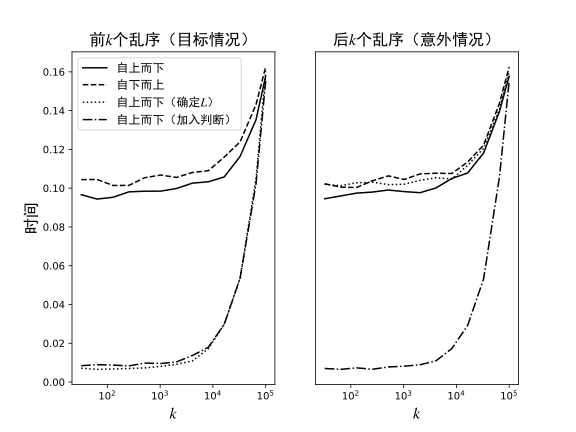
\includegraphics[width=0.7\linewidth]{figures/vec16.pdf}
  \caption{归并排序在局部乱序情况下的性能}
  \label{fig:vec16}
\end{figure}

如图\ref{fig:vec16}所示,
在本小节介绍的两种方法中,从递归方程入手的方法具有更好的\textit{泛用性}。我们可以测试一个对偶问题:有且只有后缀是乱序的问题。在这个对偶问题上,从递归方程入手的方法仍然可以做到高效率,而从递归目标入手的方法则因为无法识别先验信息,和未改进的版本性能相若。从图中还可以看出,即使是没有做针对性优化的版本,由于有序段内不需要移动后半段,在“整体有序”的情况下性能也可以得到一定的提升。

\section{有序向量上的算法}

\subsection{折半查找}
排序之后得到的有序向量,在查找时有额外的优越性。排序之后要执行查找操作,就不再需要一个一个元素看是否相等了。类似排序,我们首先建立针对有序线性表的抽象查找类。

\begin{lstlisting}
template <typename T, template <typename> typename Linear = DefaultVector>
    requires std::is_base_of_v<AbstractLinearList<T, typename Linear<T>::position_type>, Linear<T>>
class AbstractSearch : public Algorithm<typename Linear<T>::position_type(const Linear<T>&, const T&)> {
protected:
    using output_type = typename Linear<T>::position_type;
    std::function<bool(const T&, const T&)> cmp { std::less<T>() };
    virtual output_type search(const Linear<T>& L, const T& e) = 0;
public:
    template <typename Comparator>
    output_type operator()(const Linear<T>& L, const T& e, Comparator cmp) {
        this->cmp = cmp;
        return search(L, e);
    }
    output_type operator()(const Linear<T>& L, const T& e) override {
        return search(L, e);
    }
};
\end{lstlisting}

这里可以使用刚才介绍的,基于比较的算法思路。将被查找的元素$e$和向量中的某个元素$V[i]$比较,比较结果有2种:
\begin{enumerate}
    \item 如果$V[i] > e$,那么只需要保留$V[0$:$i]$作为新的查找区间。
    \item 如果$V[i] \le e$,那么只需要保留$V[i$:$n]$作为新的查找区间。
\end{enumerate}

当取$i = \frac n2$(\textbf{折半})时,可以保证新的查找区间长度大约是原来的一半,从而在$\Theta(\log n)$的时间里完成查找。所以这个思路称为\textbf{折半查找}。当然,也存在其他二分的方法($i$取其他值),参见后面的《查找》一章。

\textit{您可以借助上面的设计或者自己的理解,设计折半查找的算法。}下面给出了一个使用递归的示例代码,它实现了刚才的设计。

\begin{lstlisting}
template <typename T>
class BinarySearchRecursive : public AbstractSearch<T, DefaultVector> {
    Rank search(const Vector<T>& V, const T& e, Rank lo, Rank hi) const {
        if (hi - lo <= 1) {
            return lo < V.size() && this->cmp(V[lo], e) ? hi : lo;
        }
        Rank mi { lo + (hi - lo) / 2 };
        if (this->cmp(e, V[mi])) {
            return search(V, e, lo, mi);
        } else {
            return search(V, e, mi, hi);
        }
    }
protected:
    Rank search(const Vector<T>& V, const T& e) override {
        return search(V, e, 0, V.size());
    }
};
\end{lstlisting}

上面的算法,时间复杂度和空间复杂度均为$\Theta(\log n)$,您可以自己证明。

查找是算法设计的重点。在设计的时候,需要尤其注意多个相等元素的时候是返回秩最大、秩最小还是任意一个,以及查找失败的时候返回何种特殊值。
如果是无序向量,正如\ref{seg:查找一个元素}节那样,那么在查找失败的时候很自然地会返回一个无效值,比如说$-1$或者$V\mathrm{.size}()$。但是在有序向量的情况下,即使查找失败,我们也可以返回一些\textit{有意义}的值,向调用者传递一些额外的信息。
下面以前面的折半查找算法为例,分析查找成功和查找失败的情况下返回值的设计。

因为如果$e<V[\mathrm{mi}]$就只保留前半段$V[\mathrm{lo}$:$\mathrm{mi}]$,所以我们在任何时刻都可以保证,$V[\mathrm{hi}] > e$(可认为初始值$V[V\mathrm{.size()}] = +\infty$)。另一方面,因为另一边的比较是不严格的,所以我们保证的是$V[\mathrm{lo}]\le e$;注意,这个式子只有$\mathrm{lo}\ne 0$也就是$\mathrm{lo}$被修改过一次之后才成立。

而当进入递归边界的时候,$V[\mathrm{lo}$:$\mathrm{hi}]$有且只有一个元素$V[\mathrm{lo}]$。此时,可以分成小于、等于、大于三种情况讨论。
\begin{enumerate}
    \item 如果$V[\mathrm{lo}] < e$,那么我们可以定位到$V[\mathrm{lo}] < e < V[\mathrm{hi}]$,此时返回$\mathrm{hi}$,就是大于$e$的第一个元素。
    \item 如果$V[\mathrm{lo}] = e$,那么我们直接返回$\mathrm{lo}$,符合查找算法的期待;并且,由于$e < V[\mathrm{hi}]$,所以如果有多个等于$e$的元素,则返回的是最大的秩。
    \item 如果$V[\mathrm{lo}] > e$,根据前面的分析可知,这种情况只可能发生在$\mathrm{lo} = 0$的情况。于是,$e$小于向量中的所有元素,此时返回$\mathrm{lo}$,也是大于$e$的第一个元素。
\end{enumerate}

综上所述,我们验证了上述折半查找算法的正确性,并且在查找成功时,返回的是最大的秩,在查找失败时,返回的是大于$e$的第一个元素的秩。\textit{二分算法在设计的时候非常容易出错;当您自己设计二分算法的时候,也可以使用上面的思考流程来分析自己的算法。}

\subsection{消除尾递归}
\label{vec:消除简单尾递归}
查找$V[0$:$n]$中某个元素$e$的下标,这个问题在计算前有$n+1$种(包括$-1$)可能的结果,计算后有$1$种确定的答案,因此从信息论的角度讲,最坏时间复杂度一定是$\Omega(\log n)$的。但空间复杂度并不一定要是$\Omega (\log n)$。在这一小节,将介绍一种叫做\textbf{消除尾递归}的技术,使用这个技术,可以将上面的折半查找算法的空间复杂度降为$O(1)$。

如果一个递归函数只在返回(return)前调用自身,则称其为\textbf{尾递归}(tail recursion)。在实际的编程过程中如果开启了编译器优化选项,则尾递归在通常会被编译器自动优化。

本小节只介绍对于尾递归的消除方法,其他类型的递归消除将在后文中讨论。
对于尾递归,只需要将递归函数的参数作为循环变量,就可以将其改写为不含递归的形式,从而降低空间复杂度。下面的模板是典型的尾递归。

\begin{lstlisting}
R operator()(Args... args) override {
    if ((*pred)(args...)) {
        return (*bound)(args...);
    }
    return apply(*this, (*next)(args...));
}
\end{lstlisting}

示例代码可以在\textit{VectorSearch.cpp}中找到,这里只提取出关键部分。如果您对模板元编程的技巧不感兴趣,下面的说明略读即可。其中,需要传入三个仿函数指针\lstinline{pred}(用于判断是否进入递归边界的谓词)、\lstinline{bound}(用于在递归边界上生成返回值)和\lstinline{next}(用于在非递归边界上生成下一个递归调用的参数)。\lstinline{std::apply}用于将\lstinline{next}返回的元组再次传递到仿函数中进行调用。此外,
递归参数往往是值而不是引用。引用总是作为整个递归过程中共享的参数,如折半查找中的向量$V$和待查找元素$e$,而不是每次递归调用时传递的参数。因此,我们可以直接用值传递\lstinline{args...},而不需要使用\lstinline{std::forward}进行完美转发。
上面的递归算法可以改写成如下的迭代算法,其中\lstinline{std::tie}表示元组的绑定赋值。

\begin{lstlisting}
R operator()(Args... args) override {
    while (!(*pred)(args...)) {
        tie(args...) = (*next)(args...);
    }
    return (*bound)(args...);
}
\end{lstlisting}

\subsection{实验:迭代形式的折半查找}

您可以利用上面的尾递归模板,将折半查找递归形式进行拆解,分解出\lstinline{pred}、\lstinline{bound}和\lstinline{next},然后代入到上面的迭代模板中,\textit{将其改写为迭代形式}。示例代码仍然在\textit{VectorSearch.cpp}中。比如,\lstinline{next}可以实现为:

\begin{lstlisting}
tuple<Rank, Rank> operator()(Rank lo, Rank hi) override {
    Rank mi { lo + (hi - lo) / 2 };
    if (cmp(e, V[mi])) {
        return { lo, mi };
    } else {
        return { mi, hi };
    }
}
\end{lstlisting}

下面是迭代形式的一个示例程序,它和最初的递归形式是完全等价的。
\begin{lstlisting}
Rank search(const Vector<T>& V, const T& e) override {
    Rank lo { 0 }, hi { V.size() };
    while (hi - lo > 1) {
        Rank mi { lo + (hi - lo) / 2 };
        if (this->cmp(e, V[mi])) {
            hi = mi;
        } else {
            lo = mi;
        }
    }
    return lo < V.size() && this->cmp(V[lo], e) ? hi : lo;
}
\end{lstlisting}

在示例的测试程序中,我们构造了长度为$n$的向量,将其随机赋值为某个区间的数并排序,然后重复$10^4$次查找(这是因为单次查找的效率太高,无法正确反映各个算法的性能差异)。我们会发现,由于进行了很多抽象,使用模板的方法性能会显著低于直接递归或迭代的性能;而递归和迭代之间相差无几(编译器对递归的版本进行了自动优化)。但即使成模板,它作为对数复杂度的算法,效率仍然远远高于在\ref{seg:查找一个元素}节中讨论的顺序查找,\textit{您可以自己实现一个基于顺序查找的算法参与对比}。

在本节的最后再次强调,
现代C++编译器如果开启了优化选项,通常可以在编译的过程中自动消除尾递归,所以在实际上机编程时,不需要刻意将尾递归改写成循环形式。但在《数据结构》中分析算法的时候,不应该考虑编译器做的优化,所以在算法设计题中,如果出现了未被改写的尾递归,就会有被扣空间分的风险。此外,您也不应当总是依赖编译器的尾递归优化,因为一些语言(比如Python)拒绝提供尾递归优化~\cite{van2012tail},在C++中运行良好的代码移植到这些语言上可能会发生问题。

\subsection{实验:向量唯一化}

下面讨论\textbf{唯一化}(unique)问题。给定一个向量,我们希望删除它中间\textit{相等}的重复元素,只保留秩最小的那一个。这里再次看到了\textit{相等}和\textit{相同}的区别,数据结构中是不可能有相同的元素的,而相等的元素我们可以用它的地址(位置、秩)来区分。代码可以在\textit{VectorUnique.cpp}中找到。

\begin{lstlisting}
template <typename T>
class VectorUnique : public Algorithm<void, Vector<T>&> {};
\end{lstlisting}

一个简单但有效的解法是:从左到右考察$V$中的每个元素,删除这个元素的后缀中,所有和它相等的元素。\textit{在看下面的代码前,您可以自己实现这个算法。}

\begin{lstlisting}
// VectorUniqueBasic
void operator()(Vector<T>& V) override {
    for (Rank r { 0 }; r < V.size(); ++r) {
        V.resize(remove(begin(V) + r + 1, end(V), V[r]) - begin(V));
    }
}
\end{lstlisting}

在上面的算法里,利用了我们在\ref{sec:按值删除元素}节中使用的“删除-擦除”法一次性地删除后缀里的所有重复元素;因此,最好情况下(所有元素都相等),可以达到$\Theta(n)$的时间复杂度。虽然按值删除达到了$\Theta(n-r)$的时间复杂度,但是因为$r$需要遍历整个向量,所以在最坏情况下(即所有元素都互不相同)需要进行$\Theta(n^2)$次比较。

值得一提的是,如果按值删除的时候采用的是最坏情况$\Theta(n^2)$的朴素(逐个删除)算法,那么唯一化在最坏情况下时间复杂度仍然是$\Theta(n^2)$,并不会来到$\Theta(n^3)$。这是初学者容易出现的错误,即直接把循环内外的时间复杂度相乘。这种天真的想法可能是来自于公式$O(f(n))\cdot O(g(n)) = O(f(n)\cdot g(n))$。这个公式本身没有问题,但我们联系一下概率论里的$P(A)P(B)=P(AB)$的条件就能发现端倪:如果内层循环和外层循环是有联系的(不独立的),那么就不能直接相乘。比如,在上面的代码中,外层循环的$r$的区间是0到$V\mathrm{.size}()$;然而,$V\mathrm{.size}()$并不是一个常量$n$,在内层循环中它会发生变化。在使用朴素算法进行按值删除的时候,删除的元素越多,花费的时间越长,但同时缩小的向量规模也就越多,减少的外层循环的轮数也就越多。\textit{您可以在这个基础上,完成对朴素按值删除情况下,上述唯一化算法的时间复杂度分析。}

在有序向量的情况下,问题可以得到进一步的简化。相等的元素总是排在连续的位置的。所以,可以通过快慢指针的方法。快指针一次经过一片相等的元素,而慢指针保留这些元素中的第一个(这个算法的前提条件并不是有序,只要求相等的元素排在一起即可,但通常建立这一条件的方法是排序)。\textit{您已经见过好几次快慢指针的方法,应该可以自己写出来。}下面是一个示例程序。

\begin{lstlisting}
// VectorUniqueFSP
void operator()(Vector<T>& V) override {
    Rank r { 0 }, s { 0 };
    while (++s < V.size()) {
        if (V[r] != V[s]) {
            V[++r] = move(V[s]);
        }
    }
    V.resize(++r);
}
\end{lstlisting}

这个算法的时间复杂度是$\Theta(n)$的。在STL中,提供了\lstinline{std::unique}来进行唯一化操作,它同样要求相等的元素排在一起。\lstinline{std::unique}和\lstinline{std::remove}一样不提供擦除功能,需要再进行\lstinline{resize}。

如果定义了全序关系(即可排序),那么无序向量的唯一化可以化归到有序向量的情况进行处理:先进行一次$\Theta(n\log n)$的排序,再用有序向量唯一化。但在排序的时候,会损失“元素原先的位置”这一信息,所以需要开辟一个额外的$\Theta(n)$的空间保存这一信息,以在唯一化之后能够顺利还原。\textit{您可以尝试实现这样的算法,并和给出的示例算法相比较。}它的时间复杂度为$\Theta(n\log n)$,优于前面的VectorUniqueBasic;但需要引入辅助向量,空间复杂度为$\Theta(n)$。

\begin{lstlisting}
template <typename T>
class VectorUniqueSort : public VectorUnique<T> {
    struct Item {
        T value;
        Rank rank;
        bool operator==(const Item& rhs) const {
            return value == rhs.value;
        }
        auto operator<=>(const Item& rhs) const {
            return value <=> rhs.value;
        }
    };
    Vector<Item> W;
    void moveToW(Vector<T>& V) {
        W.resize(V.size());
        for (Rank r { 0 }; r < V.size(); ++r) {
            W[r].value = move(V[r]);
            W[r].rank = r;
        }
    }
    void moveToV(Vector<T>& V) {
        V.resize(W.size());
        for (Rank r { 0 }; r < W.size(); ++r) {
            V[r] = move(W[r].value);
        }
    }
public:
    void operator()(Vector<T>& V) override {
        moveToW(V);
        stable_sort(begin(W), end(W));
        W.resize(unique(begin(W), end(W)) - begin(W));
        sort(begin(W), end(W), [](const Item& lhs, const Item& rhs) {
            return lhs.rank < rhs.rank;
            });
        moveToV(V);
    }
};
\end{lstlisting}

\begin{figure}
  \centering
  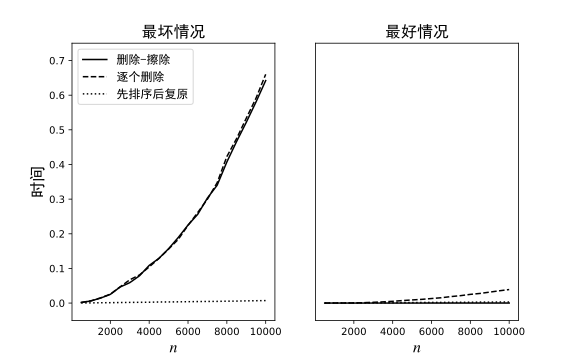
\includegraphics[width=0.8\linewidth]{figures/vec17.pdf}
  \caption{最坏和最好情况下的向量唯一化性能}
  \label{fig:vec17}
\end{figure}

如图\ref{fig:vec17}所示,
通过实验我们看到,在最坏情况下(所有元素互不相同),直接对无序向量进行处理,无论采用“删除-擦除”法还是逐个删除法都非常慢,而先排序再复原则快得多。而在最好情况下(所有元素都相同),“删除-擦除”法时间复杂度仅为$\Theta(n)$最快,先排序后复原需要$\Theta(n\log n)$较慢,而逐个删除的方法仍然需要$\Theta(n^2)$最慢。

\section{实验:循环位移}

通常我们遍历向量都采用从前向后、一个一个元素遍历的形式。
在本章的最后,用\textbf{循环位移}(cyclic shift)作为例子,讨论一下非常规的遍历方法。代码可以在\textit{CyclicShift.cpp}中找到。

给定向量$V[0$:$n]$和位移量$k$,则将原有的向量$V[0],V[1],\dots,V[n-1]$,变换为$V[k],V[k+1],\dots,V[n-1],V[0],V[1],\dots,V[k-1]$,称为\textbf{循环左移}。相应地,变换为$V[n-k],V[n-k+1],\dots,V[n-1],V[0],V[1],\dots,V[n-k-1]$,称为\textbf{循环右移}。循环左移和循环右移的实现方法大同小异,这一小节只讨论循环左移,右移的情况请您自己完成。\textit{建议您先自己设计解决这个问题的算法并实现。}

循环左移的过程可以表示为$(V[0$:$k],V[k$:$n])\to (V[k$:$n],V[0$:$k])$。这个形式非常类似于交换。相信您一定知道最经典的交换函数的实现:
\begin{lstlisting}
template <typename T>
void swap(T& a, T& b) {
    T tmp { move(a) };
    a = move(b);
    b = move(tmp);
}
\end{lstlisting}

一个最朴素的想法,就是用类似的辅助空间,暂存$V[0$:$k]$中的元素,然后通过3次移动来完成循环左移,如图\ref{fig:vec11}所示。

\begin{figure}[H]
  \centering
  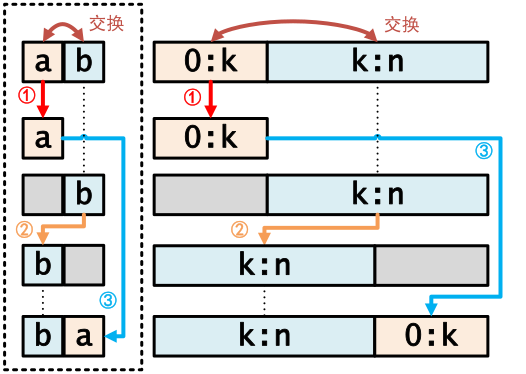
\includegraphics[width=0.8\linewidth]{figures/vec11.pdf}
  \caption{用三次移动实现循环左移,与交换元素的对比}
  \label{fig:vec11}
\end{figure}

\begin{lstlisting}
// CyclicShiftMove
void operator()(Vector<T>& V, size_t k) override {
    Vector<T> W(k);
    move(begin(V), begin(V) + k, begin(W));
    move(begin(V) + k, end(V), begin(V));
    move(begin(W), end(W), end(V) - k);
}
\end{lstlisting}

这一算法的时间复杂度是$\Theta(k)+\Theta(n-k)+\Theta(k)=\Theta(n+k)$。考虑到$k=O(n)$,也可以简化为$\Theta(n)$。空间复杂度则为$\Theta(k)$。

下面的目标则是将空间复杂度降到$O(1)$。
为了保持时间复杂度仍然为$\Theta(n)$不变,需要尽可能\textit{一步到位}地移动元素。当我们让$V[i+k]$移动到$V[i]$的位置上时,需要暂存$V[i]$到辅助空间去。下一步,如果继续将$V[i+k+1]$移动到$V[i+1]$的位置,那么需要的辅助空间就会增大。为了防止辅助空间增大,则需要考虑“不用暂存”的元素:也就是已经被移动的$V[i+k]$。下一步将$V[i+2k]$移动到$V[i+k]$的位置,这就是不需要新的辅助空间的。

因此可以得到一个算法:将$V[i+k]$移动到$V[i]$,再将$V[i+2k]$移动到$V[i+k]$,以此类推。由于向量中的元素是有限的,您可以证明,存在$j$,使得$(i+jk) \% n = i$,也就是经过$j$次移动后回到了$V[i]$。最后一次赋值,将辅助空间里的$V[i]$拿出来赋给$V[i-k]$也就是$V[i+(j-1)k]$即可。这样实现了一个“轮转交换”的功能。

需要注意的是,这样一轮并不一定能经过$V$中所有的元素。比如在$n=6, k=2, i=0$时,只轮转交换了$V[0],V[2],V[4]$这3个元素,而对另外3个元素则没有移动。我们可能需要进行多轮“轮转交换”,各轮共享同一个辅助空间。图\ref{fig:vec12}展示了$n=12,k=3$的轮转交换例子。

\begin{figure}
  \centering
  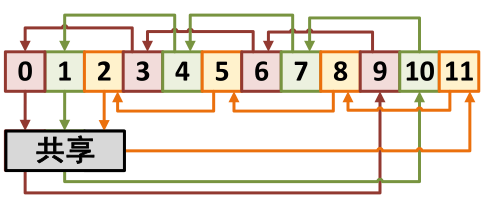
\includegraphics[width=0.8\linewidth]{figures/vec12.pdf}
  \caption{用轮转交换进行循环位移}
  \label{fig:vec12}
\end{figure}

下面证明:对任意的秩$0 \le r < n $,都存在唯一的$0 \le i < d$和$0 \le j < \frac nd$,使得$r = (i+jk) \% n$。其中,$d = \mathrm{gcd}(n,k)$是$n$和$k$的最大公因数。

\begin{proof}
因为$r$和数对$(i,j)$的取值范围都是$n$元集,所以只要证明$(i,j)$到$r$是单射,就蕴含了它同时是满射。
因此,只需要证明对于不等的$(i_1,j_1)$和$(i_2,j_2)$,$(i_1+j_1k) \%n\ne(i_2+j_2k)\%n$。

假设存在整数$q$,使得$(i_1-i_2)+(j_1-j_2)k+qn=0$。由于$(j_1-j_2)k+qn$必定是$d$的倍数,而$|i_1-i_2|<d$,所以只能有$i_1=i_2$。

设$k=k_1d,n=n_1d$,那么$(j_1-j_2)k_1+qn_1=0$。因为$(k_1,n_1)=1$,所以$j_1-j_2$必定是$n_1$的倍数,但$|j_1-j_2|<\frac nd=n_1$,所以只能有$j_1=j_2$。这和$(i_1,j_1)$与$(i_2,j_2)$不等矛盾,故由反证法得到单射成立。
\end{proof}

于是,遍历顺序应当是:依次从$0,1,\dots,d-1$出发,以$k$为步长遍历$\frac nd$次回到起点。这个算法的书写有一定挑战性,您可以效仿前面的\lstinline{swap}去实现轮转交换。

\begin{lstlisting}
// CyclicShiftSwap
void operator()(Vector<T>& V, size_t k) override {
    size_t d { static_cast<size_t>(gcd(V.size(), k)) };
    for (Rank i { 0 }; i < d; ++i) {
        T tmp { move(V[i]) };
        Rank cur { i }, next { (cur + k) % V.size() };
        while (next != i) {
            V[cur] = move(V[next]);
            cur = next;
            next = (cur + k) % V.size();
        }
        V[cur] = move(tmp);
    }
}
\end{lstlisting}

这一算法的时间复杂度是$\Theta(d)\cdot \Theta\left(\frac nd\right) = \Theta(n)$,空间复杂度降低到了$O(1)$。

在很多教材上会介绍另一种解法:三次\textbf{反转}(reverse)。基于反转的原理是,为了实现$(V[0$:$k],V[k$:$n])\to (V[k$:$n],V[0$:$k])$,本质上是需要让后半段移动到前半段,前半段移动到后半段。而反转恰好能实现这个功能,且不需要移动算法那样的额外空间。在第一次反转后,$V[0$:$n]$变为了$\overline{V}[n$:$0]$(这里用上划线表示反转),我们可以将它拆分为$(\overline{V}[n$:$k],\overline{V}[k$:$0])$,然后再将这两段分别反转即可,如图\ref{fig:vec13}所示。

\begin{figure}
  \centering
  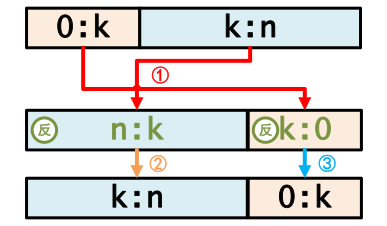
\includegraphics[width=0.5\linewidth]{figures/vec13.pdf}
  \caption{用三次反转进行循环位移}
  \label{fig:vec13}
\end{figure}

\begin{lstlisting}
// CyclicShiftReverse
void operator()(Vector<T>& V, size_t k) override {
    reverse(begin(V), end(V));
    reverse(begin(V), end(V) - k);
    reverse(end(V) - k, end(V));
}
\end{lstlisting}

\begin{table}
  \centering
  \caption{循环位移算法的耗时对比(单位:ms)}
  \begin{tabular}{ll|ccc}
    \toprule
      位移量$k,$ & $n = 10^8$ & 三次移动 & 循环位移 & 三次反转  
      \\
    \midrule
    1 & 最小值 & 2788 & 1909 & 3424 \\
    $10,000$ & 较小值 & 2769 & 2250 & 3418 \\
    $5\times 10^7$ & 中间值 & 4236 & 1869 & 3428 \\
    $9\times 10^7$ & 较大值 & 5370 & 1917 & 3442 \\
    \midrule
    $10,007$ & 素数 & 2751 & 5783 & 3439 \\
    \bottomrule
  \end{tabular}
  \label{tab:vec4}
\end{table}

三次反转的时间复杂度同样是$\Theta(n)$,而空间复杂度是$O(1)$。下面从理论层面来比较以上三种做法的时间效率。三次移动的做法,写入内存的次数为$k+(n-k)+k=n+k$。轮转交换的做法,写入次数为$n$(每个元素都一步到位地写入了目标位置)。三次反转的做法,写入次数为$n+(n-k)+k=2n$。显然,轮转交换的写入次数最少,三次移动次之,三次反转最多。但实际上,由于三次移动中开辟$\Theta(k)$的空间(并自动做零初始化)和释放本身需要时间,所以它在$k$比较大的时候反而会慢于三次反转。您可以从实验结果中看到这一点。
此外,您还能从实验结果中看到,虽然理论上轮转交换的写入次数是$n$,但它的时间消耗上下浮动很大(并不像三次移动那样随$k$变大而变大),有些时候时间消耗还会大于三次移动和三次反转。这是算法的\textit{局部性}导致的,具体机制参见《组成原理》。三次反转虽然很多时候不是速度最快的算法,但对于各种情况的$k$性能相当稳定。

最后,C++ STL提供了\lstinline{std::rotate}函数进行循环位移。根据编译器的不同,其可能会选用轮转交换或者三次反转的算法(MSVC使用的是三次反转)。您可以从实验结果中看出您的编译器使用了何种算法实现该函数。

\section{本章小结}
向量(顺序表)是程序设计中最经常使用的数据结构,因此本章具有较大的容量。向量的顺序结构是简单的,向量的循秩访问特性是自然的,无论是学习还是考试,这一章的重点都在算法设计上。本章通过较多的实验展示了一些算法设计的典型技巧。其中,对于排序和查找两个重点内容,我们还将在后续的算法章节再次讨论。

本章的主要学习目标如下:
\begin{enumerate}
    \item 您有了对算法设计中的不必要工作的优化意识。
    \item 您学会了对顺序表的整块进行操作,而不是对单个元素进行操作。
    \item 您学会了使用快慢指针进行探测和更新。
    \item 您了解到可以从信息的观点分析时间复杂度问题。
    \item 您了解到排序预处理可以为后续问题的解决提供帮助。
    \item 您了解了分析分摊复杂度和平均复杂度的意义。
    \item 您深化了对递归-迭代关系的认识,掌握了消除尾递归的方法。
\end{enumerate}

向量本身是很简单的数据结构,记忆它的插入、删除、查找和各种变形,也是相对简单的;重要的地方在于希望您能理解并掌握书中这些典型算法的设计思路、优化思路。希望本书的内容能为您解决基于向量的算法设计问题提供帮助。

% \chapter{图表示例}

% \section{插图}

% 图片通常在 \env{figure} 环境中使用 \cs{includegraphics} 插入,如图~\ref{fig:example} 的源代码。
% 建议矢量图片使用 PDF 格式,比如数据可视化的绘图;
% 照片应使用 JPG 格式;
% 其他的栅格图应使用无损的 PNG 格式。
% 注意,LaTeX 不支持 TIFF 格式;EPS 格式已经过时。

% \begin{figure}
%   \centering
%   \includegraphics[width=0.5\linewidth]{example-image-a.pdf}
%   \caption*{国外的期刊习惯将图表的标题和说明文字写成一段,需要改写为标题只含图表的名称,其他说明文字以注释方式写在图表下方,或者写在正文中。}
%   \caption{示例图片标题}
%   \label{fig:example}
% \end{figure}

% 若图或表中有附注,采用英文小写字母顺序编号,附注写在图或表的下方。
% 国外的期刊习惯将图表的标题和说明文字写成一段,需要改写为标题只含图表的名称,其他说明文字以注释方式写在图表下方,或者写在正文中。

% 如果一个图由两个或两个以上分图组成时,各分图分别以 (a)、(b)、(c)...... 作为图序,并须有分图题。
% 推荐使用 \pkg{subcaption} 宏包来处理, 比如图~\ref{fig:subfig-a} 和图~\ref{fig:subfig-b}。

% \begin{figure}
%   \centering
%   \subcaptionbox{分图 A\label{fig:subfig-a}}
%     {\includegraphics[width=0.35\linewidth]{example-image-a.pdf}}
%   \subcaptionbox{分图 B\label{fig:subfig-b}}
%     {\includegraphics[width=0.35\linewidth]{example-image-b.pdf}}
%   \caption{多个分图的示例}
%   \label{fig:multi-image}
% \end{figure}



% \section{表格}

% 表应具有自明性。为使表格简洁易读,尽可能采用三线表,如表~\ref{tab:three-line}。
% 三条线可以使用 \pkg{booktabs} 宏包提供的命令生成。

% \begin{table}
%   \centering
%   \caption{三线表示例}
%   \begin{tabular}{ll}
%     \toprule
%     文件名          & 描述                         \\
%     \midrule
%     thuthesis.dtx   & 模板的源文件,包括文档和注释 \\
%     thuthesis.cls   & 模板文件                     \\
%     thuthesis-*.bst & BibTeX 参考文献表样式文件    \\
%     \bottomrule
%   \end{tabular}
%   \label{tab:three-line}
% \end{table}

% 表格如果有附注,尤其是需要在表格中进行标注时,可以使用 \pkg{threeparttable} 宏包。
% 研究生要求使用英文小写字母 a、b、c……顺序编号,本科生使用圈码 ①、②、③……编号。

% \begin{table}
%   \centering
%   \begin{threeparttable}[c]
%     \caption{带附注的表格示例}
%     \label{tab:three-part-table}
%     \begin{tabular}{ll}
%       \toprule
%       文件名                 & 描述                         \\
%       \midrule
%       thuthesis.dtx\tnote{a} & 模板的源文件,包括文档和注释 \\
%       thuthesis.cls\tnote{b} & 模板文件                     \\
%       thuthesis-*.bst        & BibTeX 参考文献表样式文件    \\
%       \bottomrule
%     \end{tabular}
%     \begin{tablenotes}
%       \item [a] 可以通过 xelatex 编译生成模板的使用说明文档;
%         使用 xetex 编译 \file{thuthesis.ins} 时则会从 \file{.dtx} 中去除掉文档和注释,得到精简的 \file{.cls} 文件。
%       \item [b] 更新模板时,一定要记得编译生成 \file{.cls} 文件,否则编译论文时载入的依然是旧版的模板。
%     \end{tablenotes}
%   \end{threeparttable}
% \end{table}

% 如某个表需要转页接排,可以使用 \pkg{longtable} 宏包,需要在随后的各页上重复表的编号。
% 编号后跟表题(可省略)和“(续)”,置于表上方。续表均应重复表头。

% \begin{longtable}{cccc}
%     \caption{跨页长表格的表题}
%     \label{tab:longtable} \\
%     \toprule
%     表头 1 & 表头 2 & 表头 3 & 表头 4 \\
%     \midrule
%   \endfirsthead
%     \caption*{续表~\thetable\quad 跨页长表格的表题} \\
%     \toprule
%     表头 1 & 表头 2 & 表头 3 & 表头 4 \\
%     \midrule
%   \endhead
%     \bottomrule
%   \endfoot
%   Row 1  & & & \\
%   Row 2  & & & \\
%   Row 3  & & & \\
%   Row 4  & & & \\
%   Row 5  & & & \\
%   Row 6  & & & \\
%   Row 7  & & & \\
%   Row 8  & & & \\
%   Row 9  & & & \\
%   Row 10 & & & \\
% \end{longtable}



% \section{算法}

% 算法环境可以使用 \pkg{algorithms} 或者 \pkg{algorithm2e} 宏包。

% \renewcommand{\algorithmicrequire}{\textbf{输入:}\unskip}
% \renewcommand{\algorithmicensure}{\textbf{输出:}\unskip}

% \begin{algorithm}
%   \caption{Calculate $y = x^n$}
%   \label{alg1}
%   \small
%   \begin{algorithmic}
%     \REQUIRE $n \geq 0$
%     \ENSURE $y = x^n$

%     \STATE $y \leftarrow 1$
%     \STATE $X \leftarrow x$
%     \STATE $N \leftarrow n$

%     \WHILE{$N \neq 0$}
%       \IF{$N$ is even}
%         \STATE $X \leftarrow X \times X$
%         \STATE $N \leftarrow N / 2$
%       \ELSE[$N$ is odd]
%         \STATE $y \leftarrow y \times X$
%         \STATE $N \leftarrow N - 1$
%       \ENDIF
%     \ENDWHILE
%   \end{algorithmic}
% \end{algorithm}
